\documentclass[10pt,journal,compsoc]{IEEEtran}

\usepackage{ctex}
\usepackage{times}
\usepackage{epsfig}
\usepackage{graphicx}
\usepackage{amsmath}
\usepackage{amssymb}
\usepackage{hyperref}
\usepackage{enumerate}
\usepackage{enumitem}
\usepackage{caption}
\usepackage{color}
\usepackage{comment}
\usepackage{url}
\usepackage{xcolor}
\usepackage{tabu}
\usepackage{booktabs}
\usepackage{makecell}
\usepackage{wrapfig}
\usepackage{breakcites}
\usepackage{subfig}
\usepackage{ragged2e}
\usepackage{stfloats}
\usepackage{xcolor}
\usepackage[export]{adjustbox}
\usepackage{indentfirst}
\usepackage{multirow}
\setlength{\parindent}{2em} 
\usepackage{stfloats}

\usepackage{arydshln}
\usepackage{float}

\usepackage[T1]{fontenc}
\usepackage{lmodern}
\usepackage{textcomp}

\usepackage{tikz}
\renewcommand*\textcircled[1]{\tikz[baseline=(char.base)]{
            \node[shape=circle,draw,inner sep=1.2pt] (char) {#1};}}

\usepackage{algorithm}
\usepackage[noend]{algpseudocode}

% 定义代码样式
\usepackage{listings}

\definecolor{gray}{rgb}{0.96,0.96,0.96}

\lstset{ %
  language=python,                % the language of the code
  basicstyle=\footnotesize,           % the size of the fonts that are used for the code
  numbers=left,                   % where to put the line-numbers
  columns=fixed, 
  numberstyle=\tiny\color{black},  % the style that is used for the line-numbers
  stepnumber=1,                   % the step between two line-numbers. If it's 1, each line 
                                  % will be numbered
  numbersep=1.5mm,                  % how far the line-numbers are from the code
  xleftmargin=1.3em,
  backgroundcolor=\color{gray},      % choose the background color. You must add \RequirePackage{color}
  showspaces=false,               % show spaces adding particular underscores
  showstringspaces=false,         % underline spaces within strings
  showtabs=false,                 % show tabs within strings adding particular underscores
  frame=single,,                 % adds a frame around the code
  frameround = tttt,
  framexleftmargin=3mm, 
  rulecolor=\color[RGB]{158,193,243},        % if not set, the frame-color may be changed on line-breaks within not-black text (e.g. commens (green here))
%  aboveskip=1em,
  tabsize=2,                      % sets default tabsize to 2 spaces
  captionpos=b,                   % sets the caption-position to bottom
  breaklines=true,                % sets automatic line breaking
  extendedchars=false,   
  breakatwhitespace=false,        % sets if automatic breaks should only happen at whitespace
  title=\lstname,                   % show the filename of files included with \lstinputlisting;
                                  % also try caption instead of title
  keywordstyle=\color[RGB]{0,51,179},          % keyword style
  commentstyle=\color[RGB]{140,140,140},       % comment style
  stringstyle=\color[RGB]{6,125,23},         % string literal style
  identifierstyle=\color{black},
  escapeinside={\%*}{*)},            % if you want to add LaTeX within your code
  morekeywords={*,...}               % if you want to add more keywords to the set
}

\def\Plus{\texttt{+}}

\makeatletter
\def\BState{\State\hskip-\ALG@thistlm}
\makeatother

\graphicspath{{figures/}}

% *** CITATION PACKAGES ***
%
\ifCLASSOPTIONcompsoc
  % IEEE Computer Society needs nocompress option
  % requires cite.sty v4.0 or later (November 2003)
  \usepackage[nocompress]{cite}
\else
  % normal IEEE
  \usepackage{cite}
\fi

% *** GRAPHICS RELATED PACKAGES ***
%
\ifCLASSINFOpdf

\else

\fi

\hyphenation{op-tical net-works semi-conduc-tor}


\usepackage{lettrine}


\begin{document}
\begin{sloppypar}

\title{数字图像处理-理论测验}

\author{唐麒\qquad 21120299\\qitang@bjtu.edu.cn}

\IEEEtitleabstractindextext{
\begin{abstract}
\justifying 对齐向来是视频超分辨率重建(Video Super-Resilution, VSR)中的重要操作,然而自注意机制的进展可能会违背这一常识。本文重新思考了 Transformer VSR 中对齐的作用,并进行了一些反直觉的观察。实验表明,VSR Transformer 可以直接使用未对齐的多帧信息,而现有的对齐方法可能并不适用 VSR Transformer。此外,简单的移除对齐模块并采用更大的注意窗口可以进一步提高  VSR Transformer 的性能。然而,这种设计将大大增加计算负担,并不能处理大的运动。为此,本文提出了一种基于 patch 的对齐方法,该方法利用图像 patch 代替像素进行对齐并获得 SOTA 表现。

\end{abstract}

\begin{IEEEkeywords}
视频超分辨率重建、Transformer、光流
\end{IEEEkeywords}}


% make the title area
\maketitle

%\twocolumn[{%
%\renewcommand\twocolumn[1][]{#1}%
%\maketitle
%\pagenumbering{arabic}
%
%\vspace{-1.5cm}
%\noindent\begin{minipage}{\linewidth} 
% 	\begin{center}
% 	\captionsetup{font=small}
% 	\begin{tabular}{@{}c@{}c@{}c@{}}
%% 	\includegraphics[width=0.31\linewidth,cframe=red!50!black 1mm]{fig1_a} &
%% 	\includegraphics[width=0.31\linewidth,cframe=green!50!black 1mm]{fig1_b} &
%%    \includegraphics[width=0.313\linewidth,cframe=blue!50!black 1mm]{fig1_c} \vspace{-1mm}\\
%	\includegraphics[width=0.31\linewidth]{fig1_a} &
% 	\includegraphics[width=0.31\linewidth]{fig1_b} &
%    \includegraphics[width=0.32\linewidth]{fig1_c} \vspace{-1mm}\\
%    {\small (a)} &  {\small (b)}  &  {\small (c)} \\
%    \end{tabular}
%	\vspace{-3mm}
%	\captionof{figure}{\small 原始图像及三个不同阈值下的分割结果: (a) Test\_Img\_1, (b) Test\_Img\_2, and (c) Test\_Img\_3. 三个阈值分别为125(右上)、99(左下)和156(右下)}
%	\label{fig:random_thresholding}
%	\end{center}  \vspace{1.25cm}
%\end{minipage}
%}]

\IEEEraisesectionheading{\section{正交变换}
\label{sec:orthogonal_transformation}}

 \lettrine{数}{字}图像处理的方法主要分为两大类,一个是空间域处理法(或称空域法),一个是频域法(或称变换域法)。在频域法中最为关键的预处理便是变换处理,这种变换一般是线性变换。具体而言,就是将空域中的信号(图像)变换到另外一个域(频域),即使用该域中的一组单位正交基函数(相同基函数内积为1,不同基函数内积为0)的线性组合来表示任意函数。使用这组基函数的线性组合得到任意函数$f$,每个基函数的系数就是$f$与该基函数的内积。

图像变换通常是一种二维正交变换,一般要求必须是可逆的,正变换和反变换的算法不能太复杂,而且在变换域中图像能量将集中分布在低频率成分上,边缘、线状信息反映在高频率成分上。这样做可以使图像处理问题简化,有利于图像特征提取并有助于从概念上增强对图像信息的理解。因此,正交变换被广泛地运用于图像特征提取、图像增强、图像复原、图像识别以及图像编码等处理中。主要的正交变换包括傅立叶变换、离散余弦变换、沃尔什变换、哈尔变换、斜变换和小波变换。

傅里叶变换是大家所熟知的正交变换,在一维信号处理中有着广泛应用。把这种处理方法推广到图像处理中是很自然的事。通俗来讲,一维傅立叶变换是将一个一维的信号分解成若干个复指数波$e^{jwx}$。而由于$e^{jwx} =cos(wx)+jsin(wx)$,所以可以将每一个复指数波$e^{jwx}$都视为是余弦波 $+ j\times$ 正弦波的组合。一维信号是一个序列,傅立叶变换将其分解成若干个一维的简单函数之和。二维信号可以说是一个图像,类比一维,那二维傅立叶变换就是将图像分解成基图像(即复平面波$e^{ji\pi (ux+vy)}$)之和,这些基图像是相互正交的,图像变换的本质是寻找合适的基图像来表达图像。

		对图像进行二维傅里叶变换得到的频谱图,中心部分表示原图像中的低频部分,是图像中灰度变化不太快的成分,反映了图像的主体框架;频谱的四周,也即是高频区域是图像中灰度变化较快的成分,一般反映着图像中的椒盐噪声(突发性的白点或黑点)或者是图像内部变化剧烈的边缘成分。
	
	傅里叶变换的一个最大问题是它的参数都是复数,在数据的描述上相当于实数的两倍。而离散余弦变换为全实数的正交变换,能够达到和傅立叶变换相同功能但数据量又不大。二维离散余弦变换的定义由下式表示:
	
\begin{equation}
\begin{aligned}
& F(0,0)=\frac{1}{N} \sum_{x=0}^{N-1} \sum_{y=0}^{N-1} f(x, y) \\
& F(0, v)=\frac{\sqrt{2}}{N} \sum_{x=0}^{N-1} \sum_{y=0}^{N-1} f(x, y) \cdot \cos \frac{(2 y+1) v \pi}{2 N} \\
& F(u, 0)=\frac{\sqrt{2}}{N} \sum_{x=0}^{N-1} \sum_{y=0}^{N-1} f(x, y) \cos \frac{(2 x+1) u \pi}{2 N} \\
& F(u, v)=\frac{2}{N} \sum_{x=0}^{N-1} \sum_{y=0}^{N-1} f(x, y) \cos \frac{(2 x+1) u \pi}{2 N} \cdot \cos \frac{(2 y+1) v \pi}{2 N}
\end{aligned}
\end{equation}

二维离散余弦反变换的定义由下式表示:

\begin{equation}
\begin{aligned}
f(x, y) & =\frac{1}{N} F(0,0)+\frac{\sqrt{2}}{N} \sum_{v=1}^{N-1} F(0, v) \cos \frac{(2 y+1) v \pi}{2 N} \\
& +\frac{\sqrt{2}}{N} \sum_{u=1}^{N-1} F(u, 0) \cos \frac{(2 x+1) u \pi}{2 N} \\
& +\frac{2}{N} \sum_{u=1}^{N-1} \sum_{v=1}^{N-1} F(u, v) \cos \frac{(2 x+1) u \pi}{2 N} \cdot \cos \frac{(2 y+1) v \pi}{2 N}
\end{aligned}
\end{equation}

与傅里叶变换一样,离散余弦变换自然可以由定义 式出发进行计算。但这样的计算量太大,在实际应 用中很不方便。所以也要寻求一种快速算法。 首先,从定义出发,作如下推导:

\begin{equation}
\begin{aligned}
F(u) & =\sqrt{\frac{2}{N}} \sum_{x=0}^{N-1} f(x) \cos \frac{(2 x+1) u \pi}{2 N} \\
& =\sqrt{\frac{2}{N}} \sum_{x=0}^{N-1} f(x) R_e\left\{e^{-j \frac{(2 x+1) u \pi}{2 N}}\right\} \\
& =\sqrt{\frac{2}{N}} R_e\left\{\sum_{x=0}^{N-1} f(x) e^{-j \frac{(2 x+1) u \pi}{2 N}}\right\}
\end{aligned}
\vspace{0.3cm}
\end{equation}

如果把时域数据数据向量作下列延拓,即:

\begin{equation}
f_e(x)= \begin{cases}f(x) & x=0,1,2, \cdots \cdots, N-1 \\ 0 & x=N, N+1, \cdots \cdots, 2 N-1\end{cases}
\vspace{0.3cm}
\end{equation}

则 $f_e(x)$ 的离散余弦变换可写作下式:

\begin{equation}
\begin{aligned}
F(0) & =\frac{1}{\sqrt{N}} \sum_{x=0}^{2 N-1} f_e(x) \\
F(u) & =\sqrt{\frac{2}{N}} \sum_{x=0}^{2 N-1} f_e(x) \cos \frac{(2 x+1) u \pi}{2 N} \\
& =\sqrt{\frac{2}{N}} R_e\left\{\sum_{x=0}^{2 N-1} f_e(x) e^{-j \frac{(2 x+1) u \pi}{2 N}}\right\} \\
& =\sqrt{\frac{2}{N}} R_e\left\{e^{-j \frac{u \pi}{2 N}} \cdot \sum_{x=0}^{2 N-1} f_e(x) e^{-j \frac{2 x u \pi}{2 N}}\right\}
\end{aligned}
\vspace{0.3cm}
\end{equation}

可见 $\sum_{x=0}^{2 N-1} f_e(x) e^{-j \frac{2 x u \pi}{2 N}}$ 正是延拓后 $2N$ 点的离散傅立叶变换。所以在作离散余弦变换时,可以把序列长度延拓为 $2N$,然后作离散傅里叶变换,产生的结果取其实部便可得到余弦变换。同样,离散余弦反变换可以从 $\left[F_e(u) \cdot e^{j \frac{u \pi}{2 N}}\right]$ 的 $2N$ 点反傅立叶变换实现。

\begin{figure}[!ht]
	\centering
	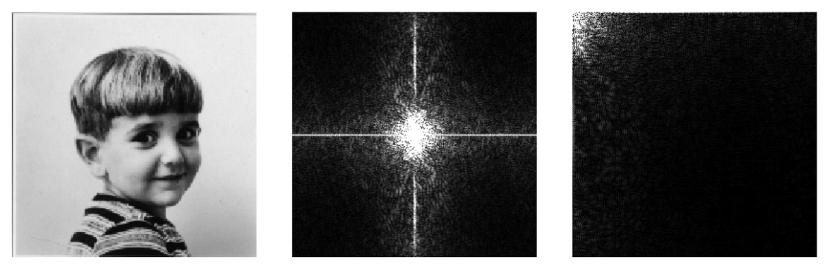
\includegraphics[width=\linewidth]{1.png}
	\caption{原始图像及快速傅立叶变换、离散余弦变换频谱图}
	\label{fig:fig1}
\end{figure}

如 \textbf{图 \ref{fig:fig1}} 所示,除了数据存储量和运算速度的差别,在变换获得的频谱图方面,离散傅立叶变换也比傅立叶变换更加集中。具体运用方面,离散余弦变换是JPEG有损压缩算法的基础(JPEG2000是基于小波变换的图像压缩标准,压缩比更高,而且不会产生基于离散余弦变换的JPEG标准产生的分块效应)。其算法流程如 \textbf{图 \ref{fig:fig2}} 所示。

\begin{figure}[!ht]
	\centering
	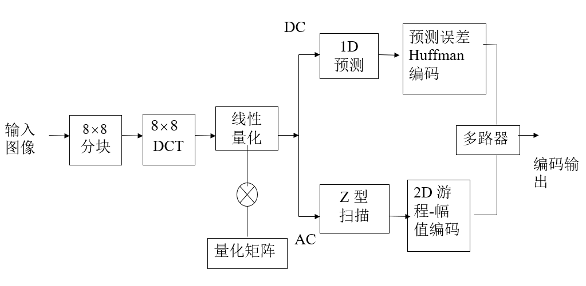
\includegraphics[width=\linewidth]{2.png}
	\caption{JPEG 基本系统压缩过程框图}
	\label{fig:fig2}
	\vspace{-0.6cm}
\end{figure}

具体来说,首先将原始图像分割成 $8\times 8$ 的子块,对于彩色图像,它要求 YUV 4:2:2格式。为消除直流电平的影响,将原始图像的所有像素减去128,再进行 DCT 变换进行去相关性。然后进行四舍五入取整,这也是图像质量下降的主要原因,JPEG 给出了量化系数矩阵表,在量化表设计时考虑了人眼的视觉特性。在编码输出时,对于直流系数预测,预测后进行熵编码;而对于交流系数,首先对交流系数进行Z型扫描,编码以游程-幅值 Huffman编码的形式完成。JPEG过程在进行分块后对每一块进行DCT变换,高压缩比时,线性量化的量化步长较大,量化后将一些高频系数变成了0,反变换后,成为了全灰的,能看到明显的方块效应。为了改善或者消除方块效应,可以用小波变化代替余弦变换,也可以降低量化步长或者在分块时 overlap,当然也可以采用后处理的方法。

正交变换一般是线性变换,其基本线性运算式严格可逆,并且满足一定的正交条件。而对于深度学习而言,更重要的是模型的非线性能力,因此直觉上来讲用深度学习的方法来做正交变换是行不通的。因此基于深度学习的正交变换主要从两个方向进行调研:基于深度学习的稀疏表示和正交变换在深度学习方法中的应用。

传统的模式识别里面,主要是对信号进行特征提取,然后对特征进行识别,这样既能减除大部分无谓的干扰,又能降低识别的运算量。提取特征最简单的方式就是正交变换,正交变换是无损的特征提取,可以在信号与特征之间互相转换。比较典型的一个应用是基于Gabor变换的纹理分析。对于纹理分析而言,采用 Gabor 滤波具有较好的时-频局部特性,它能够同时表示和捕捉二维信号在空间位置、空间频率、方向选择性和相位、频率带宽等方面的信息。用 Gabor 滤波器对图像信号滤波,相当于将其按不同方向、频段进行分解,如果计算经不同方向、频段滤波后的纹理特征,这些特征将具有明显的差异,根据这些差异就可以区分不同的纹理。正交变化具有能量集中特点,也就是能把决大部分信息集中到很小的数据量上,这个也是稀疏编码的概念。如果可以接受细微的差别,我只处理前面重要特征即可,音视频压缩也用到这个性质。

稀疏编码算法是寻找一组``超完备''\footnote{如果 $M$ 个基向量刚好可以支撑 $M$ 维的欧氏空间,则这 $M$ 个基向量是完备的。如果 $M$ 个基向量可以支撑 $D$ 维的欧氏空间,并且 $M>D$,则 这 $M$ 个基向量是过完备的(overcomplete)、冗余的。“过完备”基向量是指基向量个数远远大于其支撑空间维度。因此这些基向量一般不具备独立、正交等性质
}基向量来更高效地表示样本数据的一种无监督学习方法。稀疏编码算法的目的就是找到一组基向量 $\Phi_i$,使得我们能将输入向量 $x$ 表示为这些基向量的线性组合:

\begin{equation}
\mathbf{x}=\sum_{i=1}^k a_i \phi_i
\end{equation}

超完备基的好处是它们能更有效地找出隐含在输入数据内部的结构与模式。然而,对于超完备基来说,系数 $a_i$ 不再由输入向量 $x$ 唯一确定。

这里的“稀疏性”定义为只有很少的几个非零元素或只有很少的几个远大于零(显著不为零)的元素。要求系数 $a_i$ 是稀疏的意思就是说对于一组输入向量,我们只想有尽可能少的几个系数远大于零。选择使用具有稀疏性的分量来表示我们的输入数据是有原因的,因为绝大多数的感官数据,比如自然图像,可以被表示成少量基元素的叠加,在图像中这些基本元素可以是面或者线。

把 $m$ 个输入向量的稀疏编码代价函数定义为: 

\begin{equation}
\min _{a_i^{(j)}, \phi_i} \sum_{j=1}^m\left\|\mathbf{x}^{(j)}-\sum_{i=1}^k a_i^{(j)} \phi_i\right\|^2+\lambda \sum_{i=1}^k S\left(a_i^{(j)}\right)
\end{equation}

基向量($\Phi_i,i=1,2,…,k$)对于全部的输入向量(训练样本都是一致的),系数 $a^{(j)}_i$ 是与输入向量 $x^{(j)}$ 相对应的,由基($\Phi_i$)和输入向量($x^{(j)}$)共同决定,通过其上下标($a^{(j)}_i$)即可看出。通过最优化函数得到的 $k$ 个基向量($\Phi_i$)以及全部的输入样本在该基下的表示 $a^{(j)}_i$。此处 $S(\cdot)$ 是一个稀疏代价函数,由它来对远大于零的 $a_i$ 进行“惩罚”。稀疏编码的每一维都可以被看作一种特征。和基于稠密向量的分布式表 示相比,稀疏编码具有更小的计算量和更好的可解释性等优点。


自编码器是通过无监督的方式来学习一组数据的有效编码(或表示),自编码器的结构可分为两部分:编码器和解码器。假设有一组 $D$ 维的样本 $\boldsymbol{x}^{(n)} \in \mathbb{R}^D, 1 \leq n \leq N$, 自编码器将这组数据映射到 特征空间得到每个样本的编码 $z^{(n)} \in \mathbb{R}^M, 1 \leq n \leq N$, 并且希望这组编码可以重 构出原来的样本。这一过程有点儿类似于正交变换的正变换和逆变换,与之不同的是这一过程不是线性的,也就导致逆变换得到的结果是与原信号不同的,但其目的是要尽可能重构出原来的信号。

更进一步,如果特征空间的维度 $M$ 小于原始空间的维度 $D$,自编码器相当于是一种降 维或特征抽取方法.如果 $M \geq D$,一定可以找到一组或多组解使得 $f \circ g$ 为单位函数(Identity Function),并使得重构错误为 0。然而这样的解并没有太多的意义,但是,如果再加上一些附加的约束,就可以得到一些有意义的解,比如编码 的稀疏性、取值范围,$f$ 和 $g$ 的具体形式。

在应用方面,正交变换的作用可以分为两种,一是降低模型的计算开销,二是在频率域对图像进行特征提取和模型训练。Li \cite{DBLP:conf/ijcnn/LiYR18} 等提出采用卷积定理将空域中的卷积转换为频域中的乘积的神经网络,可用于图像超分辨率重建。该网络在测试中计算效率非常高,而且其参数通过误差反向传播来进行学习,并且由于使用Hartley变换替代傅立叶变换,因此没有复数运算。Michael等 \cite{DBLP:conf/cvpr/RamamonjisoaFWL21} 受到小波分解可以实现的稀疏表示的启发提出了一种替代网络表示,使用小波分解进行更有效的深度 估计,称之为 Wavelet-Monodepth。深度图像通常由许多分段的平坦区域组成,平坦区域之间的深度有一些“跳 跃”。这种结构非常适合小波。低频分量可以代表整个场景结构,而高频分量可以很好地捕捉“跳跃”。至关重要的是,高频分量是稀疏的,这意味着计算只能集中在某些区域。这具有节省运行时计算的效果,同时仍然能够估计高质量的深度。Zhongwei Qiu等 \cite{DBLP:conf/eccv/QiuYFF22} 提出时空-频率Transformer来解决视频压缩过程中由于分块、正交变换和量化编码产生的高频伪影对视频超分辨率重建的影响。具体来讲就是利用离散余弦变换获得图像的频谱,将原始 Transformer 中 token 的划分转变为在频谱图上的划分,从而充分利用时空-频率的相关信息来完成压缩视频的超分辨率重建。


\section{图像增强} 
\label{sec:image_enhancement}

图像增强是指按特定的需要突出一幅图像中的某些信息,同时削弱或去除某些不需 要信息的处理方法。其主要目的是使处理 后的图像对某种特定的应用来说,比原始 图像更适用。因此,这类处理是为了某种应用而去改善图像质量。处理的结果使图像更适合于人的视觉特性或机器识别系统。增强处理不能增强(加)原始图像的信息,其 结果只是增强对某种信息的辨别能力,而这种处理有可能损失一些其他信息。图像增强是数字图像处理的基本内容之一。本文将以低光照图像增强为研究对象,对其传统方法和基于深度学习的方法进行调研。

图像作为感知世界的重要媒介,其质量往往决定了算法的性能。然而在图像捕获过程中,往往存在多种不可控的物理因素,导致图像质量受损,进而影响了高层视觉任务应用过程中信息的获取与利用,如人脸识别、语义分割等。在多种影响图像质量的因素当中,低光照因素较为常见且难以避免,例如阴天、夜晚等场景。为了在低光照环境下获得肉眼可见且信息丰富的高质量图像,一种直接的方式是通过物理成像过程的参数设置来提高成像质量。但单纯依赖物理成像过程的调整依然难以获得理想的图像。因此构建智能化算法以提升图像质量,已成为低光照图像增强领域的研究热点之一。

\textbf{图 \ref{fig:fig3}} 展示了不同场景下的低光照图像,从人眼的观测角度来看,几乎无法获取到有价值的信息,尤其是对于极具挑战的例子而言。事实上对于计算机而言,在这些肉眼不可见的矩阵数据中,其数值上存在的差异性是反映图像信息的关键。换言之,人眼不可见只是片面的感受,而计算机能够从图像的数值分布层面的差异和联系出发,对图像有更加清晰的认知。总之,如何利用机器学习算法实现肉眼可见的信息转换是现有低光照图像增强技术的基本目的。

\begin{figure}[!ht]
	\centering
	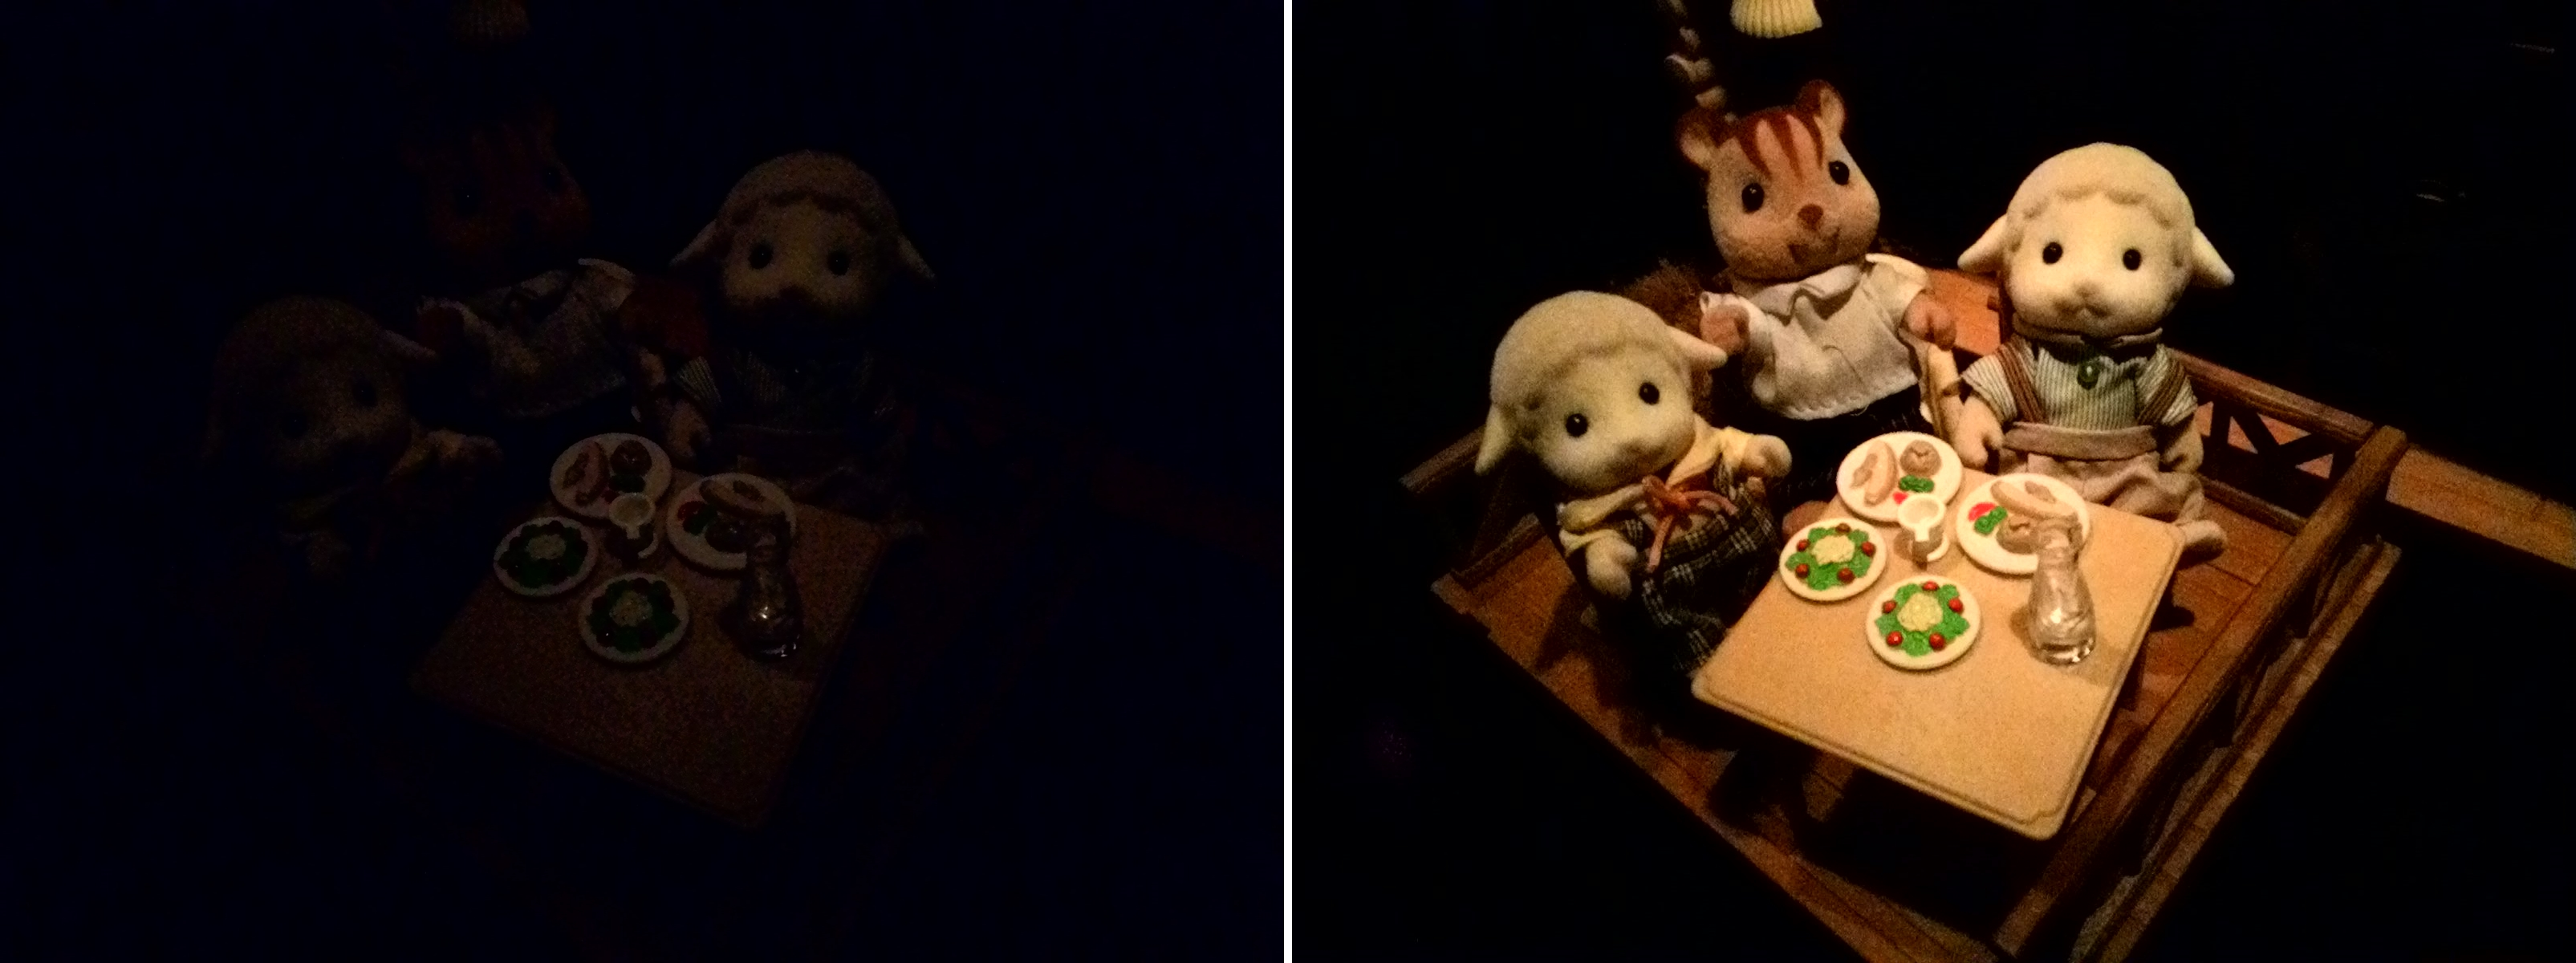
\includegraphics[width=\linewidth]{3}
	\caption{低光照图像示例}
	\label{fig:fig3}
\end{figure}

根据算法设计理念不同,现有的低光照图像增强算法可分为3类,即基于分布映射的方法,基于模型优化的方法和基于深度学习的方法。其中,基于分布映射的方法关注低光照观测的像素分布情况,致力于利用曲线变换、直方图均衡化等手段改善图像的像素分布,从而提高图像亮度与清晰度。此种类型技术与问题本身的成像过程无关,由于缺乏对于低光照图像自身对于光照需求的建模以及忽略了分布内在的联系,以致于无法有效区分语义,进而导致该类技术生成的结果往往存在颜色失真以及细节异常等视觉不友好的现象。基于模型优化的方法隶属于经典的图像处理技术范畴,其核心在于以物理成像规律导出的数据项作为基本成分,以设计刻画目标变量的正则项作为关键,并进一步利用现有的优化技术进行求解获得基于迭代的算法流程。然而,限于设计的先验的刻画能力,这些传统算法往往会产生曝光不足、色彩不饱和以及伪影或噪声明显的问题。

为了克服上述传统方法的弊端,受大数据时代的影响,通过启发式设计网络结构建立低光照输入与增强输出之间的关系,已成为一种主流的低光照图像增强模式。多种端到端的深度学习技术被设计来解决低光照图像增强任务。其中,引入特定任务的物理原理和先验正则项成为网络结构设计的主流思想。最具代表性的数据驱动型深度网络构建了“三阶段”架构。首先通过分解网络粗略估计了初始光照和反射,然后分别采用设计的架构进一步优化了这两个组件,但是,这种方式容易引起过度曝光现象,因此Retinex理论被进一步考虑以解决过曝问题。然而实际上,该过程严格执行基于模型优化的求解步骤,忽略了深度网络自身的强大推理能力。此外一些工作致力于构建低光照输入与清晰图像之间的显式连接,由于缺乏对于物理规律的利用,往往不可避免地产生其他衍生的影响视觉质量的因素。


\noindent\textbf{基于分布映射的方法}~映射低光照输入的分布以放大较小的值(显示为暗)是解决低光照图像增强的一种最直观的思路。直方图均衡化和基于S型曲线的方法是此类方法的两种代表性工作。常规的直方图均衡化方法生成结果往往会存在曝光不当、细节损失和颜色失真等问题。为此,设计了一系列基于直方图均衡化的改进版本以改善上述缺点。例如,Kim \cite{kim1997contrast} 开发了双直方图均衡化方法,Wang 等 \cite{DBLP:journals/tce/WangCZ99} 设计了二元子图像直方图均衡化方法来实现曝光的自然化处理。为了处理细节损失,Pizer 等 \cite{pizer1987adaptive} 构造了自适应直方图均衡方法,Pisano 等 \cite{DBLP:journals/jdi/PisanoZHDJMBP98}设计了对比度自适应的直方图均衡化方法。然而,由于分布映射过程中缺乏对于语义信息的识别与利用,现有的基于分布映射的方法仍然存在颜色失真等影响增强结果观感的现象。

伽玛校正是最著名的基于S型曲线的图像亮度校正技术之一,它具有映射亮度水平以补偿显示设备的非线性亮度的功能。然而对于低光照图像增强而言,伽马校正的增强结果极其不自然且不真实,尤其是在曝光水平和细节表现上。为了克服这些问题,一系列改进版本相继提出。在Bennett和McMillan \cite{DBLP:journals/tog/BennettM05} 的方法中,使用双边滤波分解低光观测,随后采用不同参数设置的S型曲线方法处理分解层,并进行重新组合。Yuan和Sun \cite{DBLP:conf/eccv/Yuan012}提出试图对通过分割输入而生成的每个子区域执行S型曲线功能。总体而言,现有的基于S型曲线的方法,曝光不均匀现象仍然是存在的最大的问题。

\noindent\textbf{基于模型优化的方法}~Retinex理论 \cite{land1971lightness} 为增强弱光图像的过程提供了直观的物理描述。该理论假设可以通过去除低光输入的光照来获得期望的正常图像(即反射图)。Retinex理论表明低光照图像与正常图像存在点除关系,其中正常图像可通过低光照图像点除根据低光照图像生成的光照图像获得。

Jobson等人 \cite{DBLP:journals/tip/JobsonRW97a} 基于Retinex理论进行了一些基本的尝试,通过引入滤波器进行光照的估计,但获得了不符合真实自然图像分布的结果,出现了未知的伪影以及色偏等现象。考虑到在一些复杂场景下,噪声和伪影始终伴随着增强过程,因此Li等人 \cite{DBLP:journals/tip/LiLYSG18} 构建了一种基于Retinex的联合低光照增强和去噪的模型,并通过定义不同的先验约束来建立优化目标。然而,由于先验约束不强以及复杂的求解过程,这项工作时常会产生过度平滑和亮度不足的结果。

随着研究的深入,研究者们发现采用Retinex模型来实现亮度提升的关键在于光照层估计。Guo等人 \cite{DBLP:journals/tip/GuoLL17} 构建了第1个只考虑对光照进行建模并求解的工作,所提出方法命名为LIME,通过使用保留边缘的平滑方法RTV(relative total variation) \cite{DBLP:journals/tog/XuYXJ12} 优化了从输入得到的初始光照。不可否认的是,该项工作取得了显著的性能,亮度突出且结构明显。但是在大多数情况下会出现曝光过度的现象。为解决LIME存在的过曝现象,Zhang等人 \cite{DBLP:conf/mm/ZhangYXZZ18, DBLP:journals/tmm/ZhangNZXZ21}从不同角度引入了一系列的光照约束,成功地将过曝现象解决,但由于引入更多的正则项约束,导致算法求解过程复杂,其推理速度显著变慢。

总体而言,对于以上基于模型优化的方法,如何设计先验正则项是大部分工作的核心,其设计过程往往依赖于一系列对于现实环境的假设条件,先验表征能力有限。此外,已有工作始终需要针对实际情况进行手动调整诸多模型参数。因此这些基于模型的工作无法在某些具有挑战的场景中实现一致优异的性能。更重要的是,基于模型优化的方法往往使用迭代过程,因此相对耗时,不利于实际应用。


\noindent\textbf{基于深度学习的方法}~从实现目的来看,基于深度学习的低光照图像增强方法能够粗略地分为两类,用于亮度增强的方法以及联合亮度增强与噪声去除的方法。以下将从这两方面展进行介绍。

1) 用于亮度增强的方法。低光照图像增强的一个核心任务在于提升图像亮度以显示更多结构与细节,因此一系列专注于亮度增强的工作相继提出。早期的工作由于成对数据的匮乏,普遍采用合成数据的方式来进行深度网络的训练。Shen等人 \cite{DBLP:journals/corr/abs-1711-02488}将卷积神经网络与Retinex理论相结合,将多尺度Retinex看做是具有跳跃链接或者是残差形式的级联高斯卷积,设计出一个多尺度的卷积神经网络MSR-net(multi-scale Retinex network),并基于Photoshop处理后的成对数据获得端对端低光照图像增强网络。网络中采用对数变换的方式将Retinex模型由相乘的形式转换为相加。由于对数变换会抑制亮区域梯度的变化,该方法容易引起细节丢失。Li等人 \cite{DBLP:journals/prl/LiGPP18}提出了一种用于低光照图像增强的卷积神经网络(LightenNet)。他们通过基于Retinex理论创建的训练对来训练设计的网络结构,但是该方法仍然难以获得令人满意的增强效果,尤其是在一些有挑战性的真实场景。

2) 联合亮度增强与噪声去除的方法。以上提及的低光照图像增强算法着重于对于亮度的提升,忽略了对于一些恶劣场景下捕获图像存在的噪声问题。为提供更高的视觉质量,现有的主流工作将同时实现亮度增强与噪声去除作为低光照图像增强的核心。Lore等人 \cite{DBLP:journals/pr/LoreAS17}设计了一种低光照网络(low-light net,LLNet)深度自动编码器,在提高低光照图像对比度的同时兼顾去噪。但由于合成数据的不真实性,导致这种方法增强后的图像会不符合实际,且存在曝光不足的问题。除了关注于网络结构的启发式设计以外,一部分工作考虑引入额外信息来辅助实现低光照图像增强。Fan等人 \cite{DBLP:conf/mm/FanWY020}将额外的先验信息引入低光照图像增强任务中。该方法将语义分割网络与Retinex方法相结合,将语义分割的结果直接作用于反射层估计网络,间接作用于低光照图像增强。除了使用语义标签之外,Zhu等人 \cite{DBLP:conf/aaai/ZhuPCY20}将图像的边缘信息引入到低光照图像增强网络中,提出了一种边缘增强多重曝光融合网络。

此外也存在一些利用其他新颖技术来实现联合亮度增强与噪声去除的工作。Zhu等人 \cite{DBLP:conf/aaai/ZhuPCY20}提出了一种新颖的三分支卷积神经网络。与之前基于Retinex的方法略有不同,该网络将图像分解为3个分量,分别是光照、反射和噪声。在网络训练过程中,通过使用迭代最小化损失函数进行权重更新。Lim和Kim \cite{DBLP:journals/tmm/Lim021}利用拉普拉斯金字塔在图像空间和特征空间中的有用性,提出了一种称为深度堆叠拉普拉斯恢复(deep stacked Laplacian restorer,DSLR)的方法。该方法能够同时生成用于亮度提升的光照信息和用于结构增强的细节信息,并在图像空间中逐步整合光照和细节信息。由于特征空间中定义的拉普拉斯金字塔基于多尺度结构中高阶残差的丰富连接,使得恢复过程更加高效。Xu等人 \cite{DBLP:conf/cvpr/0010YYL20}构建了具有真实噪声的低光照图像数据集以及对应的清晰图像。基于此数据集,提出了一种基于频率的分解和增强模型,以同时实现噪声抑制和细节增强。

考虑到现有成对数据训练机制产生的泛化性能不足,以及现有成对数据自身存在的不精确性,一系列减轻对于成对数据依赖的工作相继提出。生成对抗网络(generative adversarial network,GAN) \cite{DBLP:conf/nips/LiuBK17}是一种代表性的非成对数据训练网络,且已在一系列图像到图像(如黑夜到白天)的转换中取得显著成功。因此一个直接的想法是,GAN可以用于解决低光照图像增强问题。Shi等人 \cite{DBLP:journals/corr/abs-1906-06027}提出了一个生成器,并利用转换的SID数据集 \cite{DBLP:conf/cvpr/ChenCXK18}来实现成对数据训练。但是,由于训练过程中过于关注分布,经常导致增强的结果看起来是不自然的。为了使得恢复出的增强图像更加自然,Guo等人 \cite{DBLP:conf/cvpr/GuoLGLHKC20}通过逐步推导构造出了一种像素级别的曲线估计卷积神经网络Zero-DCE(zero-reference deep curve estimation),并设计了一系列的零参考训练损失函数,以解决低光照图像增强问题。进一步地,Li等人 \cite{DBLP:journals/pami/LiGL22}提供了加速的版本Zero-DCE++,显著提升运算效率,性能几乎保持不变。最近,在注意力机制的启发下,Jiang等人 \cite{DBLP:journals/tip/JiangGLCFSYZW21}建立了一个具有自我注意力机制的生成对抗网络,并且以一种不成对的GAN的方式进行训练。尽管该方法的性能要远优于现有的一系列基于GAN的低光增强方法,但是由于忽略了物理原理的作用,该方法在增强过程中总是会产生一些未知的伪像。Zhang等人 \cite{DBLP:journals/corr/abs-2002-11300}通过设计多种与基于模型优化的方法相关的训练损失函数,并基于RetinexNet的体系结构进行重新设计与调整,进而建立了一个自监督学习的卷积神经网络,以同时输出光照和反射。

现有低光照图像增强技术在方法层面上已经完成从传统模型设计到数据驱动的深度学习的跨越。在学习机制方面,正在从全监督学习迈向半监督/无监督学习;在应用场景方面,从相对简单的场景逐步转向更加具有挑战的真实场景(如手机拍摄);从评估方式来看,现有技术正在渐渐地跳出基于视觉质量的感知评估体系,而愈发关心下游高层视觉任务的性能,逐步从只关注视觉质量转变为高层视觉任务性能优先。此外,随着视频在生活中越来越常见,现有的工作也在逐步从空间上的图像层面转变为时序上的图像层面,即视频处理。

\section{图像编码}
\label{sec:image_encode}

图像编码属于信源编码范畴,其特点是利用图像 信号的统计特性及人眼的生理和心理特性对图像 进行高效编码。信源编码的主要任务是解决有效性问题,也就是对信源实现压缩处理,使处理后的信号更适宜数字通信系统。解决有效性问题就是在编码过程中尽量提高编码效率,也就是力求用最少的数码传递最大的信息量。

编码是信息处理科学中的经典研究课题,就图像编码而言,已有七十余年的历史。M.Kunt提出了第一代、第二代编码的概念。M.Kunt把1948-1988年这四十年中研究的以去冗余 为基础的编码方法称为第一代编码,如:PCM、 DPCM、$\Delta$M、亚取样编码法,变换域的DFT、DCT、 Walsh-Hadamard变换编码等方法以及以此为基础的 混合编码法均属于经典的第一代编码法。第二代编码方法多是八十年代以后提出的编码方法, 如金字塔编码法、Fractal编码、基于神经元网络 的编码、小波变换编码、模型基编码等。现代编码法的特点是:\textcircled{1} 充分考虑人的视觉特性;\textcircled{2} 恰当地考虑对图像信号的分解与表述;\textcircled{3} 采用图像的合成与识别方案压缩数据率。随着多媒体技术的发展已有若干编码标准由ITU-T 制定出来,如JPEG、H.261、H.263、H.264、MPEG1、 MPEG2、MPEG4、MPEG7、MPEG2000、JBIG(二值图像 压缩) 等。在第一部分的正交变换中,已经对传统方法的JPEG基本系统压缩过程及其优劣进行了介绍。这一部分将主要介绍基于深度学习的图像编码方法的进展。

\begin{figure*}[!ht]
	\centering
	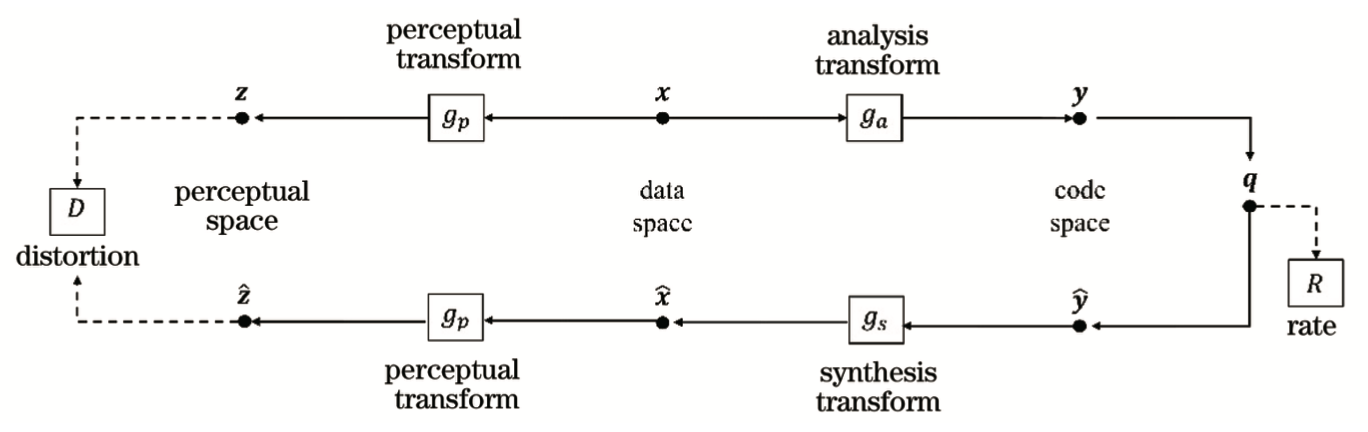
\includegraphics[width=\linewidth]{4.png}
	\caption{基于非线性变换的端到端学习图像编码框架}
	\label{fig:fig4}
\end{figure*}

前期应用神经网络技术的图像视频编码方法主要优化压缩框架中的编码工具,其主要思路都是 将 传 统 混 合 编 码 框 架和 混 合 视 频 编 码 框 架 (HVC) 中 的 模 块 与 神 经 网 络 相 结 合 来 提 升 性 能 , 但基于模块改进的性能提升有限且实现复杂。因此有必要采用端到端学习来实现整体性能的提升以满足日益增长的压缩需求。基于端到端学习的图像编码研究是从 Balé \cite{balle2016end, DBLP:conf/pcs/BalleLS16, balle2018variational}、Toderici \cite{toderici2015variable, toderici2017full}、Theis \cite{theis2017lossy} 等 的 研 究 开 始 的。最初的研究在端到端学习的压缩框架中引入了基于 CNN 或者 RNN 的自编码器,实现了可观压缩率下图像编码的整体优化重建。为了更好地表达图像相关性,研究者们一方面拓展研究了多种不同结构的自编码器,包括变分自编码器(VAE)、多尺度 自 编 码器 (MSAE)等 ,另 一 方 面 引 入 超 先 验 信 息 进 行 融 合 预 测 以 提 升 端 到 端 学 习 能 力 。 Ballé 等证 明了超先验模型中率失真优化可等效为最小化数据分 布 的 KL 散 度 (Kul lback-Leibler divergence), Zhou等 \cite{zhou2019end}提出了基于注意力机制的超先验自编码器。可见大多数基于端到端学习的图 像编码方法都依赖于自编码器的训练,以充分利 用空间相关性和数据统计分布,可在码率和失真 之间取得良好的平衡,并且可以针对任意失真指 标进行快速优化,拥有可媲美甚至超过现有国际 图 像 编 码 标 准 (如 JPEG、JPEG2000、HEVC Intra 等)的压缩性能。

除上述框架的创新外,神经网络技术也被拓展应用于图像编码中的变换、量化、熵编码等核心模块 以提升性能。变换从传统的线性离散余弦变换 (DCT)和小波变换逐步发展到非线性变换,如广义 分歧归一化(GDN)变换。在端到端学习框架中,变 换 等 效 为 利 用 逐 层 卷 积 来 提 取 特 征 激 活 (fmaps); 量化由标量量化逐步发展到矢量量化,实现从 round 函 数 到 现 在 流 行 的 软 量 化和 格 型 矢 量 量 化,这 样 可 在 满 足 数 据 压 缩 的 同 时 保 证 反 向 传 播 梯 度 可 导 ;熵 编 码 从 最 初 JPEG 使 用 的 Huf fman 编 码,发 展 到 基 于 超 先 验 和 递 归 近 邻 概 率 混 合 预 测的算术编码,实现编码性能的大幅提升; 此外, 损失函数从广泛使用的 L1损失和 L2损失,发展到改善收敛不稳定和局部最优解问题的交叉熵损 失以 及 改 善 图 像 主 观 质 量 的 感 知 损 失和对 抗 损 失,再 到 现 在 的 复 合 损 失 函 数。下面将主要对基于端到端学习的图像编码框架中这三个模块的研究现状及进展进行介绍,并对各模块中使用的方法进行了分析与对比。

\noindent\textbf{变换}~图像变换编码将空域图像像素转换为变换域系数,实现能量聚集的紧致表达,以达到压缩的目的。 大多数压缩方法都使用正交线性变换来降低数据的 相关性。在传统的变换方法中,最早针对信号冗余 解耦优化的线性变换可以追溯至 KL变换和主成分 分析法(PCA)。之后国际图像编码标准JPEG 和JPEG2000 分 别 使 用 的 离 散 余 弦 变 换 和 小 波 变 换 也 均为线性变换。

但是正交线性变换中线性滤波器响应的联合统计量呈现了很强的高阶依赖性,为解决此问题可联合局部非线性进行增益控制。近几年,端到端学习将非线性变换融入图像压缩框架中。其中,Balé 等 \cite{balle2016end, DBLP:conf/pcs/BalleLS16}提出了基于非线性变换编码的端到端学习框架,如\textbf{图\ref{fig:fig4}}所示,将图像强度向量x 先通过分析变换$y= g_a(x;\phi)$(其中 $\phi$ 为学习参数向量)映射到编码域, 再通过量化处理得到离散值向量 $q$,之后进行熵编码,相对应地,由离散值向量 $q$ 估计连续值向量 $\hat{y}$,应 用 生 成 变 换 $\hat{x}=g_s(\hat{y};\theta)$ ( 其 中 $\theta$ 为 学 习 参 数 向 量),并进行像素重建;编码决策通过率失真优化性能 ,常 见 的 失 真 度 量 包 括 均 方 误 差 (MSE)和 SSIM ,也可引入感知失真等进行性能优化,最后端到端学 习系统通过优化学习参数向量 $\phi$ 和 $\theta$ 来最小化码 率$R$和失真$D$的加权和 $R+\lambda D$ ,其中,$\lambda$控制码率 和失真的平衡。分析变换分为三个阶段:卷积、下采 样和 GDN 变换,作为其逆变换的生成变换也分为 三个阶段:仿射卷积、上采样和 GDN 逆(IGDN)变 换,且两类变换中的上下采样操作均可通过卷积来 实现,从而提高了计算效率。感知变换中归一化拉 普拉斯金字塔模型(NLP)与 GDN 的组合考虑了图像局部亮度和对比度的误差,相较于采用MSE 优化 DCT 的传统方法而言,在相似重建质量的情况下,降低了码率。

现今,自编码器被越来越广泛地用于图像压缩 中。这些研究利用单个自编码器或循环自编码器在 瓶颈层生成fmaps,用于后续的量化和熵编码 \cite{liu2018deep}。 典型的自编码器结构包含三个部分:编码器、表示压 缩数据的瓶颈和解码器,将这三个部分级联并进行 端到端训练。由于传统JPEG 等算法中线性变换对 空间相关性和压缩数据分布的利用不够充分,使用 深度卷积神经网络可实现非线性变换,对图像分布 进行更好的冗余解耦,实现更紧致的特征表达并实 现更好的压缩 \cite{theis2017lossy, zhao2018multiple, zhao2019learning, li2018learning}。

传统自编码器结构复杂、时间复杂度高,受 Shi 等 \cite{shi2016real}的工作启发,Theis等 \cite{theis2017lossy}提出基于卷积神经网 络的压缩式自编码器(CAE),对图像先进行卷积以 提取特征再进行上采样,并在解码器中采用了子像 素结构,该方法适用于高分辨率图像压缩并可大幅 度提升计算效率。对于图像编解码而言,可以通过 级联多个卷积神经网络进行定义分析和生成变换, 并允许以端到端学习的方式联合优化非线性的编码 器和解码器。因此绝大多数研究都采用了不同的卷 积神经网络进行非线性变换的设计,如 Zhao等 \cite{zhao2019learning} 利用由 CNN 组成的特征描述神经网络(FDNN)在 低维空间对真实图像(ground-truthimage)进行有 效的描述以大幅减少图像所包含的数据量,Li等 \cite{li2018learning} 用多个卷积层定义了非线性分析变换。 

综上,基于端到端学习的图像编码框架中的变 换方法从先前的正交线性变换发展到非线性变换。 现有的图像变换编码的主要作用在于提取特征以进 行更紧致的表达,且使用深度卷积神经网络的自编 码器是如今变换编码的主流方法

\noindent\textbf{量化}~在传统的图像压缩框架中,量化参数与图像质 量和码率(压缩率)息息相关。而在端到端学习的图 像压缩框架中,量化将变换后的特征激活值由浮点 数转换为规则定点数,作为后续熵编码的输入。最 常用的规则量化方法是取整函数———round函数。

由于目标失真函数主要使用梯度下降法优化端 到端编码中的率失真,反向传播中要求量化函数全 局可导,所以基于端到端学习的图像压缩研究一 直围绕着解决量化的不可导问题(量化不连续,其导 数在 任 何 地 方 都 为 零 或 无 穷 大)而 展 开。Ballé 等 \cite{balle2016end, DBLP:conf/pcs/BalleLS16}使用加性均匀噪声源代替了标量量化器实现 全局可导。

\begin{equation}
\begin{gathered}
\hat{\boldsymbol{y}}_i=\boldsymbol{q}_i=\operatorname{round}\left(\boldsymbol{y}_i\right), \\
P_{q_i}(n)=\left(p_{y_i} * \operatorname{rect}\right), n \in \mathbf{Z},\\
\widetilde{y}_i=\boldsymbol{y}_i+\Delta \boldsymbol{y}_i, \\
p_{\widetilde{y}_i}=p_{y_i} * \operatorname{rect}=\int_{n-\frac{1}{2}}^{n+\frac{1}{2}} p_{y_i}(t) \mathrm{d} t, n \in \mathbf{Z}, \\
p_{y_i}(n)=P_{q_i}(n), n \in \mathbf{Z},
\end{gathered}
\end{equation}

式中: $i$ 为索引, 遍历向量中的所有元素; $\boldsymbol{y}_i$ 为图片强 度向量 $\boldsymbol{x}_i$ 经过分析变换后的结果; $\hat{\boldsymbol{y}}_i$ 和 $\boldsymbol{q}_i$ 为 $\boldsymbol{y}_i$ 经 过量化后得到的向量; $n$ 指第 $n$ 个量化区间; $P_{q_i}$ 为 $\boldsymbol{q}_i$ 的概率质量函数; $p_{y_i}$ 为 $\boldsymbol{y}_i$ 的密度; * 代表连续卷 积; rect 为 $\left[-\frac{1}{2}, \frac{1}{2}\right]$ 的均匀分布; $\Delta \boldsymbol{y}_i$ 为均匀噪声 源, 即 rect; $\tilde{\boldsymbol{y}}_i$ 为加上均匀噪声后的 $\boldsymbol{y}_i$ 。

采用取整函数的量化将浮点数转换为整数,会 显著地降低重建的图像质量,因此 Agustsson等 \cite{agustsson2017soft} 在图像压缩的背景下探讨了矢量量化,提出软到硬 (soft-to-hard)的量化方法,让网络结合权重学习量 化级,将其应用于更广泛的问题中,并证明了矢量量 化比标量量化更具优势。传统的矢量量化需要占据 大量的存储空间且需要进行复杂的近邻搜索,对编 码器复杂度要求过高,因此 Zhao等 \cite{zhao2018multiple}提出多描述 格型矢量量化,应用对称结构避免了复杂的邻搜索。 由此可知,为解决量化的不可导问题,最常见的 方法是随机近似和用光滑导数近似的round方法。 如今矢量量化相较于标量量化成为更具竞争力的量 化方法,提出的软矢量和格型矢量的量化方法可在 保证重建质量的同时又使模型具有可微性。

\noindent\textbf{熵编码}~熵编码通过减少统计冗余进一步提升图像压缩 率。早期的深度熵编码算法能够使压缩性能得到一 定的提升,但在基于端到端学习的超先验模型出现 后,熵编码能够提供的压缩性能愈来愈高。

常用的 熵 编 码 大 多 是 变 长 编 码(VLC),其 中 包括 Huffman编码和算术编码 \cite{rissanen1981universal}。就现有的国际 图像编码标准而言,除使用 Huffman编码的JPEG 以外,其余的国际图像标准都选择使用算术编码, 目前算术编码因其可以在一个定义良好的上下文 中表现出更高的压缩率且能将量化后的fmaps转 化为 码 流 的 优 点,已 成 为 更 具 竞 争 力 的 熵 编 码 选择。

基于端到端学习的图像压缩的重要组成部分之 一是用于隐式表达的可训练熵模型,因为隐式表达 的实际分布是未知的,熵模型提供了通过近似分布 来估计编码隐式表达所需比特的方法,从而显著提 高了基于神经网络的图像压缩性能 \cite{lee2018context}。熵模型是 由 Ballé等 \cite{balle2016end}和 Theis等 \cite{theis2017lossy}首次提出的,他们的工 作对之后的研究做出了极大的贡献。前者认为隐式 表达的熵模型为非参数模型,而后者采用 GSM 模 型,其共同点在于尽可能地学习统计分布。为减少 先验和边缘信息的不匹配,Ballé等 \cite{balle2018variational}在先前研究 的基础上,通过在隐式表达的局部尺度参数上引入 超先验来捕获空间依赖性,得到更好的模型匹配,从 而增强熵模型、提升压缩性能。他们根据输入自适 应估计表达尺度,并使用 GSM 的方法将压缩的超 先验作为辅助信息添加到生成的码流中,从而允许 解码器使用条件熵模型。同年,受概率生成模型的 启发,Minnen等 \cite{minnen2018joint}提出了包含超先验和递归近邻 概率融合的自编码器,如图4所示,以两种方式扩展 了基于 GSM 的熵模型:一是将 GSM 模型推广至 GMM,在不增加模型复杂度的情况下呈现出更好 的率失真性能;二是将递归模型与超先验模型相结合。这两种结构可以互补,从而更好地利用隐式表 达的概率结构。近期,Oktay等 \cite{oktay2019scalable}又提出了一种基 于端到端学习的神经网络权值的压缩方法,该方法 先在隐式空间进行重参数化,在训练过程中采用概 率模型对参数表示施加熵惩罚,完成训练后使用 算术编码压缩隐式表达。

\begin{figure*}[!ht]
	\centering
	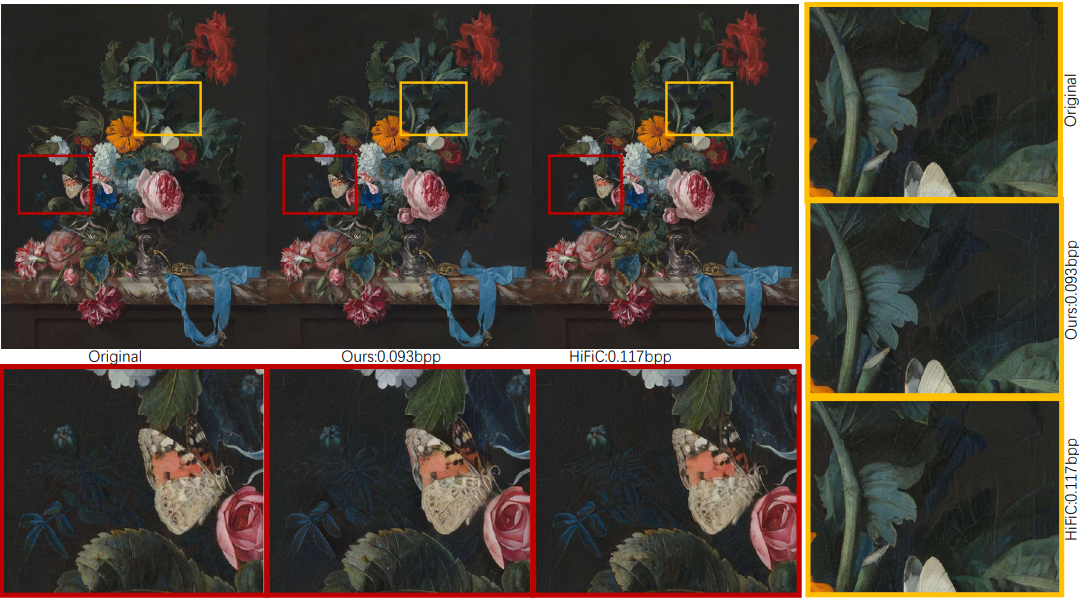
\includegraphics[width=\linewidth]{6.png}
	\caption{低比特率下 PO-ELIC 和 HiFiC 的可视化结果}
	\label{fig:fig6}
\end{figure*}

\begin{figure}[!ht]
	\centering
	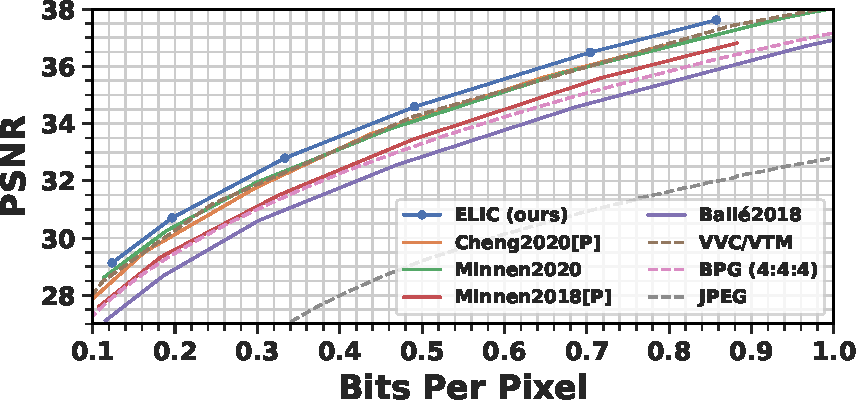
\includegraphics[width=\linewidth]{5-1.pdf}
	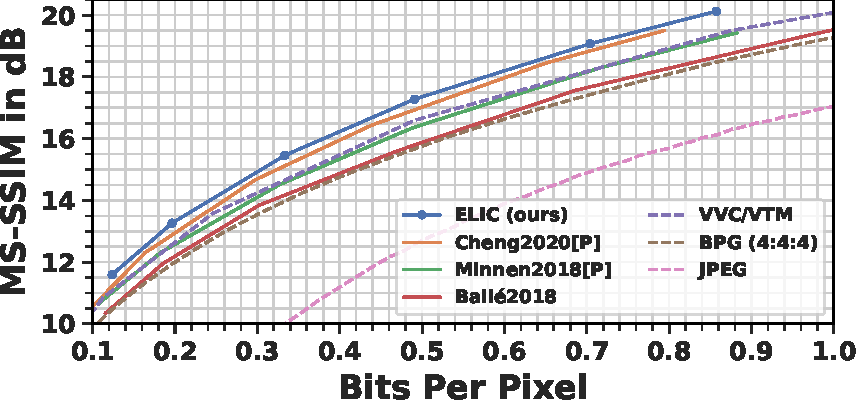
\includegraphics[width=\linewidth]{5-2.pdf}
	\caption{图像压缩方法的率失真曲线}
	\label{fig:fig5}
\end{figure}


在 Ballé等的研究基础上,Lee等 \cite{lee2018context}发现压缩 性能在本质上是取决于熵模型的容量的,因此为扩 大熵模型的容量,提出了一种上下文自适应熵模型 的框架,根据是否需要额外的比特分配,使用两种类 型的上下文:比特消耗上下文和无比特消耗上下文。 通过使用以上熵模型来更准确地估计每个隐式表达 的分布,从而更有效地减少相邻隐式表达之间的空 间依赖性,达到提高性能的目的,该研究实现的图像 压缩 性 能 在 PSNR 和 多 尺 度 结 构 相 似 性 (MS- SSIM)方面优于图像压缩的国际标准 BPG。

 综上所述,传统图像压缩框架的熵编码基本都 是 Huffman编码和算术编码,后者相较于前者而言 能够准确地呈现概率分布,更能逼近香农提出的理 论熵值。随着超先验的加入,结合了神经网络和算 术编码的混合熵模型因为有着能够近似分布、估计 编码隐式表达所需的比特以及克服隐式表达分布未 知的问题这几个优势,因此被广泛应用于基于端到 端学习的图像编码框架中。

与传统的图像编码技术相比,深度学习在训练 的阶段因其需要大量的数据量而呈现巨大的计算量 和较高的时间复杂度。而现有的应用(如云计算)可 以进行并行化,采用多 GPU 可实现数据和模型的 并行,加速深度学习的训练。训练好的模型复杂度 相对较低,硬件技术的发展和高效深度学习架构的 设计 \cite{chen2019eyeriss}有望实现实时图像编解码。同时,如今众多 的移动设备,如华为 Mate30、苹果iPhone都已经全 面支持深度学习模块,极大地促进了基于学习的图 像编解码的实际应用。除运算量这一评价指标外, 图像质量是如今图像编码研究中的主要评价指标。但无论是从数据指标还是图像质量而言,深度学习的方法均超过了传统方法。如 \textbf{图 \ref{fig:fig5}} 所示, ELIC \cite{he2022elic} 将非均匀分组模型与已有的上下文模型相结合,在不影响运行速度的情况下提高了编码性能,达到了最先进的速度-压缩率联合表现。PO-ELIC \cite{he2022po} 可以在更低的比特率下取得和 HiFiC \cite{mentzer2020high} 相当的主观感知质量,其可视化对比结果如 \textbf{\ref{fig:fig6}} 所示。

基于端到端学习的图像编码的研究只有短短几 年的历史,尽管已经取得卓越性能,但仍有较多环节 需进一步改进和完善:1)在网络结构方面,应进一步 探索新的神经网络模型在图像编码上的应用效果, 如InceptionNet、可 变 性 卷 积 等;2)在 码 率 分 配 方 面,可进一步根据图像内容差异性、特征图的分布 等,研究自适应的码率分配,以保证将码率更多地分 配在对视觉质量影响大的信息上;3)在性能方面,目 前的研究更注重压缩比和重建质量的提升,忽略了 对计算复杂度的研究和优化,但在实际应用中复杂 度是不可忽略的性能指标,因此,不仅需要研究深度 学习方法复杂度的客观衡量标准,还应以此为指导, 简化网络,实现更高效的计算;4)在硬件加速方面, 应充分考虑硬件实现的需求,对网络进行改造,从而 为将来的图像压缩芯片提供基础;5)在应用方面,随 着智能化需求的增加,图像更多地被应用于计算机 视觉,因此,可以研究图像压缩和计算机视觉之间的 共通特性,探索更有利于计算机理解和识别的图像 压缩方法。


\section{图像复原}
\label{sec:image_restoration}

图像复原是图像处理的另一重要课题,其主要目的 是改善给定图像的质量。当给定了一幅退化或受噪声污染的图像后,利用退 化现象的某种先验知识来重建或恢复原有图像是图 像复原处理的基本过程。这一部分以图像超分辨率重建为研究对象,对传统方法和基于深度学习的方法进行调研。

超分辨率图像重建利用已知的图像信息建立 LR图像与 HR 图像之间的特征序列关系,其数学模型为:利用``系统成像模型''自身的一些变化手段对退 化后的图像实现重建。``系统成像模型''过程:LR 图像由 HR 图像经退 化 函 数( 如 加 噪 、模 糊 、运 动 、降 采 样 等 )作 用 后 得 到 的不清晰图像,即:

\begin{equation}
\begin{aligned}
& D\left(I_{\mathrm{HR}} ; \theta_a\right)=\boldsymbol{S}_d \boldsymbol{B}_\kappa \boldsymbol{M} \boldsymbol{I}_{\mathrm{HR}}+n_{\xi}\{\boldsymbol{\kappa}, \xi, d\} \\
& I_{\mathrm{LR}}=D\left(I_{\mathrm{HR}} ; \theta_a\right)
\end{aligned}
\end{equation}

其中, $I_{\mathrm{LR}}$ 表示 LR 图像, $I_{\mathrm{HR}}$ 表示 $\mathrm{HR}$ 图像, $D$ 表示退 化函数, $\theta_a$ 表示与退化函数相关的各种参数和退化 因子, $S_d$ 为降采样矩阵, $d$ 为降采样矩阵的比例因 子, $\boldsymbol{B}$ 为模糊矩阵, $\kappa$ 为与 $\mathrm{HR}$ 卷积相关的模糊核, $\boldsymbol{M}$ 为运动矩阵, $n_{\xi}$ 为添加的带有标准差的噪声, $\xi$ 表示 标准差。

超分辨率图像重建问题为“系统成像模型”的逆 过程,输入 LR 图像重建出相应的 HR 图像:

\begin{equation}
I_{\mathrm{HR}}=R\left(I_{\mathrm{LR}} ; \sigma_a\right)
\end{equation}

其中, $R$ 表示重建函数, $\sigma_a$ 表示与重建函数相关的 各种参数与重建因子。图像退化过程和图像重建过程如 \textbf{图 \ref{fig:fig7}} 所示。黑色箭头表示图像退化过程,黄色箭头 表示图像重建过程。

\begin{figure}[!t]
\centering
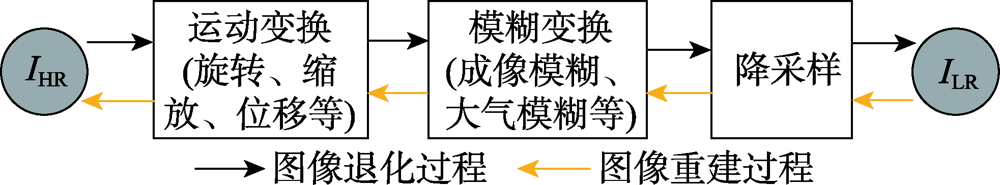
\includegraphics[width=\linewidth]{7.png}	
\caption{图像超分辨率重建技术图解}
\label{fig:fig7}
\end{figure}

\begin{figure*}[!b]
\centering
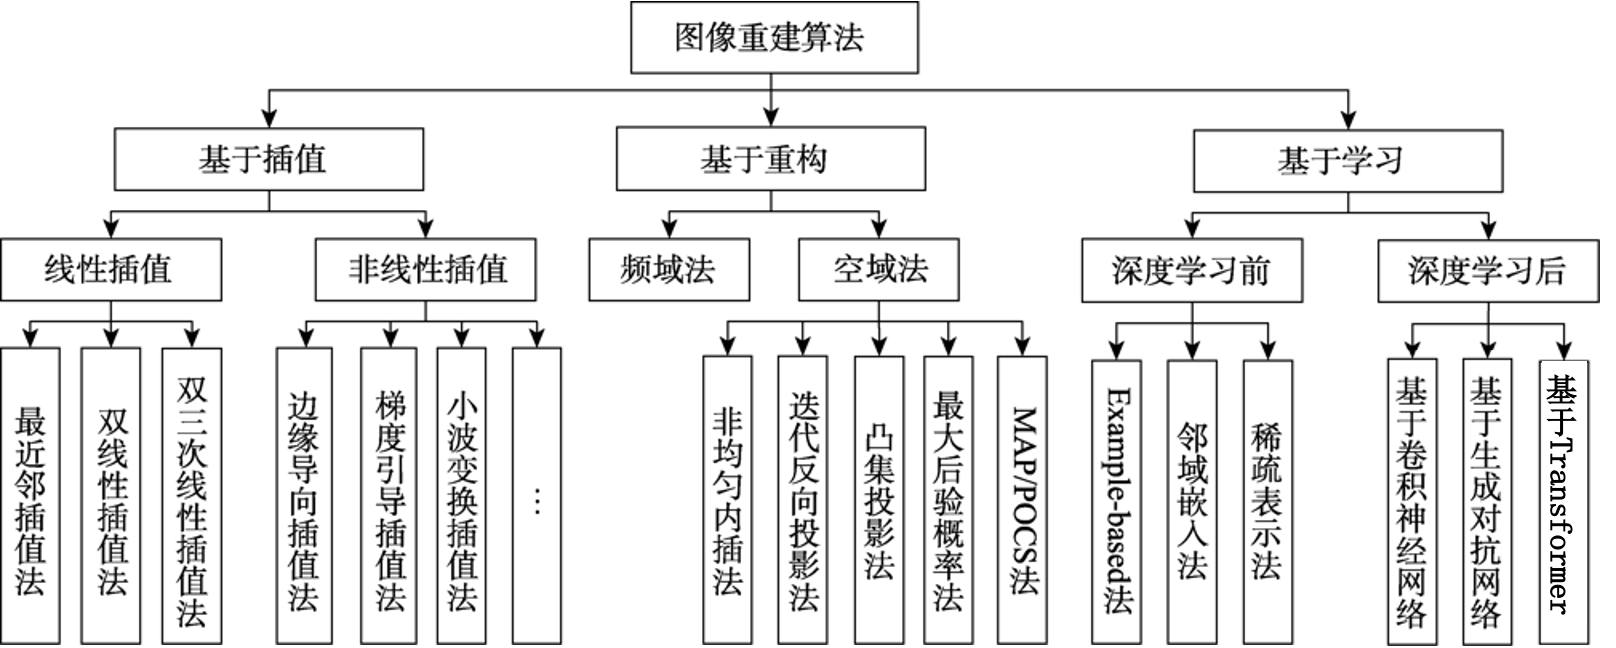
\includegraphics[width=\linewidth]{8.png}	
\caption{图像超分辨率重建方法分类}
\label{fig:fig8}
\end{figure*}


根据超分辨图像重建所采用的方法,将其 分为基于插值的图像重建方法、基于重构的图像重 建方法、基于学习的重建方法,而基于学习的图像重 建方法又可分为深度学习前的图像重建算法和深度 学习后的图像重建算法。深度学习后的图像重建算 法又分为基于卷积神经网络的超分辨率图像重建算 法、基于生成对抗网络的超分辨率图像重建算法和基于 Transformer 的超分辨率图像重建算法, 具体分类情况如 \textbf{图 \ref{fig:fig8}} 所示。本文将重点介绍基于插值的图像重建方法和基于卷积神经网络的深度学习图像重建方法。

\noindent\textbf{基于插值的图像重建方法}~基于插值的图像重建方法是超分辨率图像重建问题中最原始、最直观的方法,主要分为线性插值算 法和非线性插值算法。插值法主要根据 LR 图像已 知的像素点灰度信息,运用插值公式增强像素点间 的灰度信息来实现图像放大问题。一般情况下,插 值法所需的图像信息较少,算法复杂度较低,运行速 度较快,且插值后的 HR 图像保留了原 LR 图像的像 素点信息。基于插值的图像重建方法又包括线性插值算法和非线性插值算法两种。

\begin{enumerate}
	\item 线性插值算法
	\begin{itemize}
		\item \textbf{最近邻插值法}指插值点直接以与其欧式距 离最短的像素点的灰度值为自身插值后的灰度值。虽然它是最简单的插值算法,难度系数低且易实现, 但由于其他相邻像素点没有对目标插值点产生影 响,当插值图像分辨率较大时,容易出现锯齿效应和 图像灰度不连续问题。
		\item \textbf{双线性插值法}是为解决最近邻插值法忽视相邻像素点间影响而造成图像锯齿效应现象所提出的。双 线性插值法主要从垂直、水平两个方向对相邻的四 个像素点进行线性插值实现图像插值问题。虽然双 线性插值法在图像灰度不连续问题上有所改进,但 插值后的图像产生明显的细节退化,图像高频信息 受到损坏。
		\item \textbf{双三次插值法}是在双线性插值法的基础上提出的,将临近区域内四个相邻像素点扩充到十六个相邻像 素点,对其使用三次插值多项式后进行加权平均计 算完成图像插值重建。双三次插值法充分考虑了各 像素点对目标插值点的影响,提高了重建质量也使 计算变复杂,运算量急剧增加。
	\end{itemize}
	\item 非线性插值算法
	\begin{itemize}
		\item \textbf{边缘导向插值法}主要是对 RGB 三色图像的 边缘信息进行约束、放大,以便解决人眼视觉特性对 图像边缘信息的捕捉造成的影响。
		\item \textbf{梯度引导插值法}是利用邻域内一阶梯度、二 阶梯度的信息调整梯度分布和像素分布,再结合边 缘导向插值法和双三次线性插值法实现图像重建。
		\item \textbf{小波变换插值法}充分利用小波变换所具有 的局部细化特点,将图像特征信息分解到不同尺度 上独立研究与分析后,将提取的特征信息叠加融合 后再用小波逆变换提高图像分辨率。
	\end{itemize}
\end{enumerate}

\textbf{表 \ref{tab:tab1}} 给出了基于插值方法的各重建算法之间的 比较。基于插值的图像重建方法虽然简单且容易实 现,但图像重建效果并不理想。其中,单幅图像的重 建速度和重建效果尚且能够满足部分领域的需求, 但多幅图像的图像重建不能解决其在运算速度、运 算复杂度以及图像精度上所存在的问题。

\begin{table}[!ht]
\centering
\caption{基于插值的图像重建算法比较}
\begin{adjustbox}{width=\linewidth}
\begin{tabular}{llcccc}
\toprule
	算法 &  原理 &  运算复杂度 &  运算速度 &  算法灵活性 &  图像质量 \\ \hline
	 最近邻域插值法 &  线性插值 &  低 &  快 &  强 &  差 \\ \hline
	 双线性插值法 &  线性插值 &  较低 &  较快 &  较强 &  较差 \\ \hline
	 双三次线性插值法 &  线性插值 &  中 &  慢 &  弱 &  一般 \\ \hline
	 边缘导向插值法 &  非线性插值 &  中 &  慢 &  较强 &  高 \\ \hline
	 梯度引导插值法 &  非线性插值 &  高 &  慢 &  较弱 &  中 \\ \hline
	 小波变换插值法 &  非线性插值 &  高 &  较慢 &  中 &  高 \\ \bottomrule
\end{tabular}
\end{adjustbox}
\label{tab:tab1}
\end{table}

基于重构的超分辨率图像重建方法在图像处理领域使用较为广泛,主要分为频域法和空域法。利 用多幅 LR 图像与未知 HR 图像提取所需的图像特征 信息,并估计 HR 图像特征信息后重建 HR 图像,本文不再详细介绍。值得一提的是Irani 等人 \cite{DBLP:journals/cvgip/IraniP91}提出迭代反向投影法(iterative back- projection approach,IBP)解决超分辨率图像重建算 法对图像先验信息的高依赖性问题,有效改善重建 图像质量问题和对图像先验信息依赖问题,这一思想也被广泛应用于基于深度学习的图像(包括深度图像、多帧图像)重建方法,并取得了非常好的重建效果。

由于深度学习在计算机视觉、自然语言处理、数 据挖掘、机器翻译等领域有着较好的应用。对此,不 少学者将深度学习与 SRIR 结合,使得 SRIR 技术从最 初小规模的三层训练模型到如今大规模的深层训练 模型,运算速度、图像精度、网络结构深度都发生了 质与量的变化。且深度学习在超分辨率图像重建问题中的应用结果表明:该类型算法不仅是从深层次 网络结构去改变对图像特征的提取与重建,而且还 解决了网络结构加深所带来的过拟合、梯度消失或 爆炸、模型参数量急剧增加、网络不收敛或不稳定、 参数不能自我优化等问题,使得图像获得多尺度、多 细节的图像信息。

通常,基于深度学习的超分辨率图像重建算法 是在原有的基础网络上融入新的网络结构。比如: 多个残差块堆叠而成的残差网络,多个跳跃长(短) 连接与残差块组建的密集连接网络,多个递归单元 组成的递归神经网络,集中学习各个通道特征、层特 征、空间特征的注意力机制,加强图像连续性学习、 传递的记忆力机制以及低频信息与高频信息共享权 重的反馈机制,如\textbf{图 \ref{fig:fig9}} 所示。\textbf{表 \ref{tab:tab2}} 以表格的形式呈现出基于深度学习的超分 辨率图像重建算法深层次网络结构的类型、相关作 用和使用这些网络结构的代表算法。本文调研的方法主要为基于卷积神经网络的深度学习图像 重建算法,即直接对 LR 图像和 HR 图像进行端到端映射学习,弥补以往算法对高频细节信息丢失的缺陷, 同 时 简 化 其 学 习 过 程。

\begin{figure*}[!h]
	\centering
	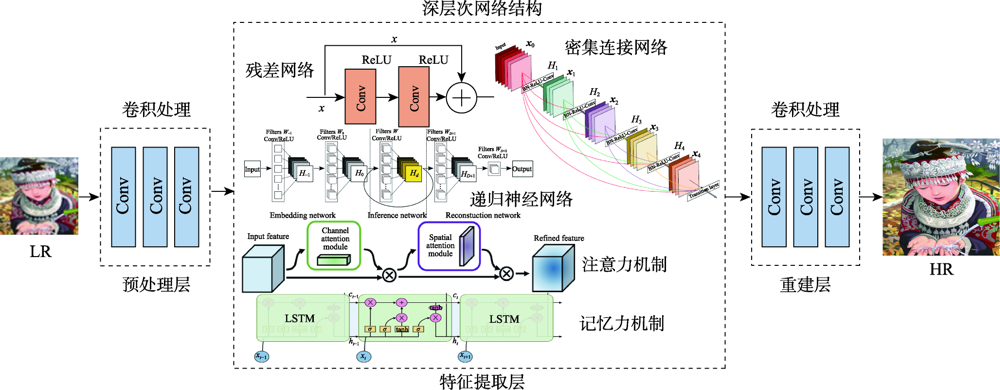
\includegraphics[width=\linewidth]{9.png}
	\caption{深度学习背景下的图像重建网络结构基本图}
	\label{fig:fig9}
\end{figure*}

\begin{table*}[!ht]
\centering
\caption{深度学习背景下的部分网络结构}
\begin{adjustbox}{width=\linewidth}
\begin{tabular}{ccc}
\toprule
	类型 &  作用 &  代表算法 \\ \hline
	 残差学习 &  提高网络收敛速度,学习丰富的复杂特征等 &  VDSR、DRCN、RDN、EDSR等 \\ \hline
	 递归学习 &  缓解梯度爆炸或消失,多路径递归学习等 &  DRCN、DRRN、SRFBN、CDC等 \\ \hline
	 密集连接 &  加强不同层之间的图像传播、利用、融合等 &  SRFBN、SRDenseNet、ESRGAN等 \\ \hline
	 跳跃连接 &  增强层间联系以及特征信息流的传递等 &  DRCN、SRDenseNet、EDSR等 \\ \hline
	 注意力机制 &  标定图像重点与非重点学习重建区域,充分挖掘层内特征信息等 &  RCAN、CBAM、SMSR、CDC、SA-SR-GAN、HAN等 \\ \hline
	 连续记忆机制 &  全局性图像特征融合,连续记忆性传递低频、高频特征信息等 &  RDN、DRRN、SRFBN、SRGAN等 \\ \hline
	 反馈机制 &  共享权重值,确保高级信息与低级信息间的表达与交流等 &  SRFBN、SRGAN、ESRGAN、SRFeat等 \\ \bottomrule
\end{tabular}
\end{adjustbox}
\label{tab:tab2}
\end{table*}

Dong 等人 \cite{DBLP:conf/iccvw/YoonJYLK15}首次将卷积神经网络与超分辨率图像重建技术结合,提出 SRCNN 算法。通过大量卷积 对输入的 LR 图像进行特征提取,不断学习众多图像 的特征表达形式,其重建效果与重建效率远超以往 的图像重建算法,且模型的泛化能力也更强。随后研究者们提出了一 系列不断优化的算法模型,从最早的基于卷积神经网络的 SRCNN(super-resolution convolutional neural net- work)模型,到基于生成对抗网络的 SRGAN(super- resolution generative adversarial network)模型 \cite{DBLP:conf/cvpr/LedigTHCCAATTWS17},再到 基 于 最 新 的 Transformer 的 TTSR(texture trans- former network for SR)模型 \cite{DBLP:conf/cvpr/YangYFLG20},基于深度学习的图像 超分重建技术不断取得新的突破。

\begin{figure*}[!hb]
  \centering
  \begin{minipage}[b]{\linewidth} 
    \subfloat[]{
    \begin{minipage}[b]{0.24\linewidth}
      \centering
      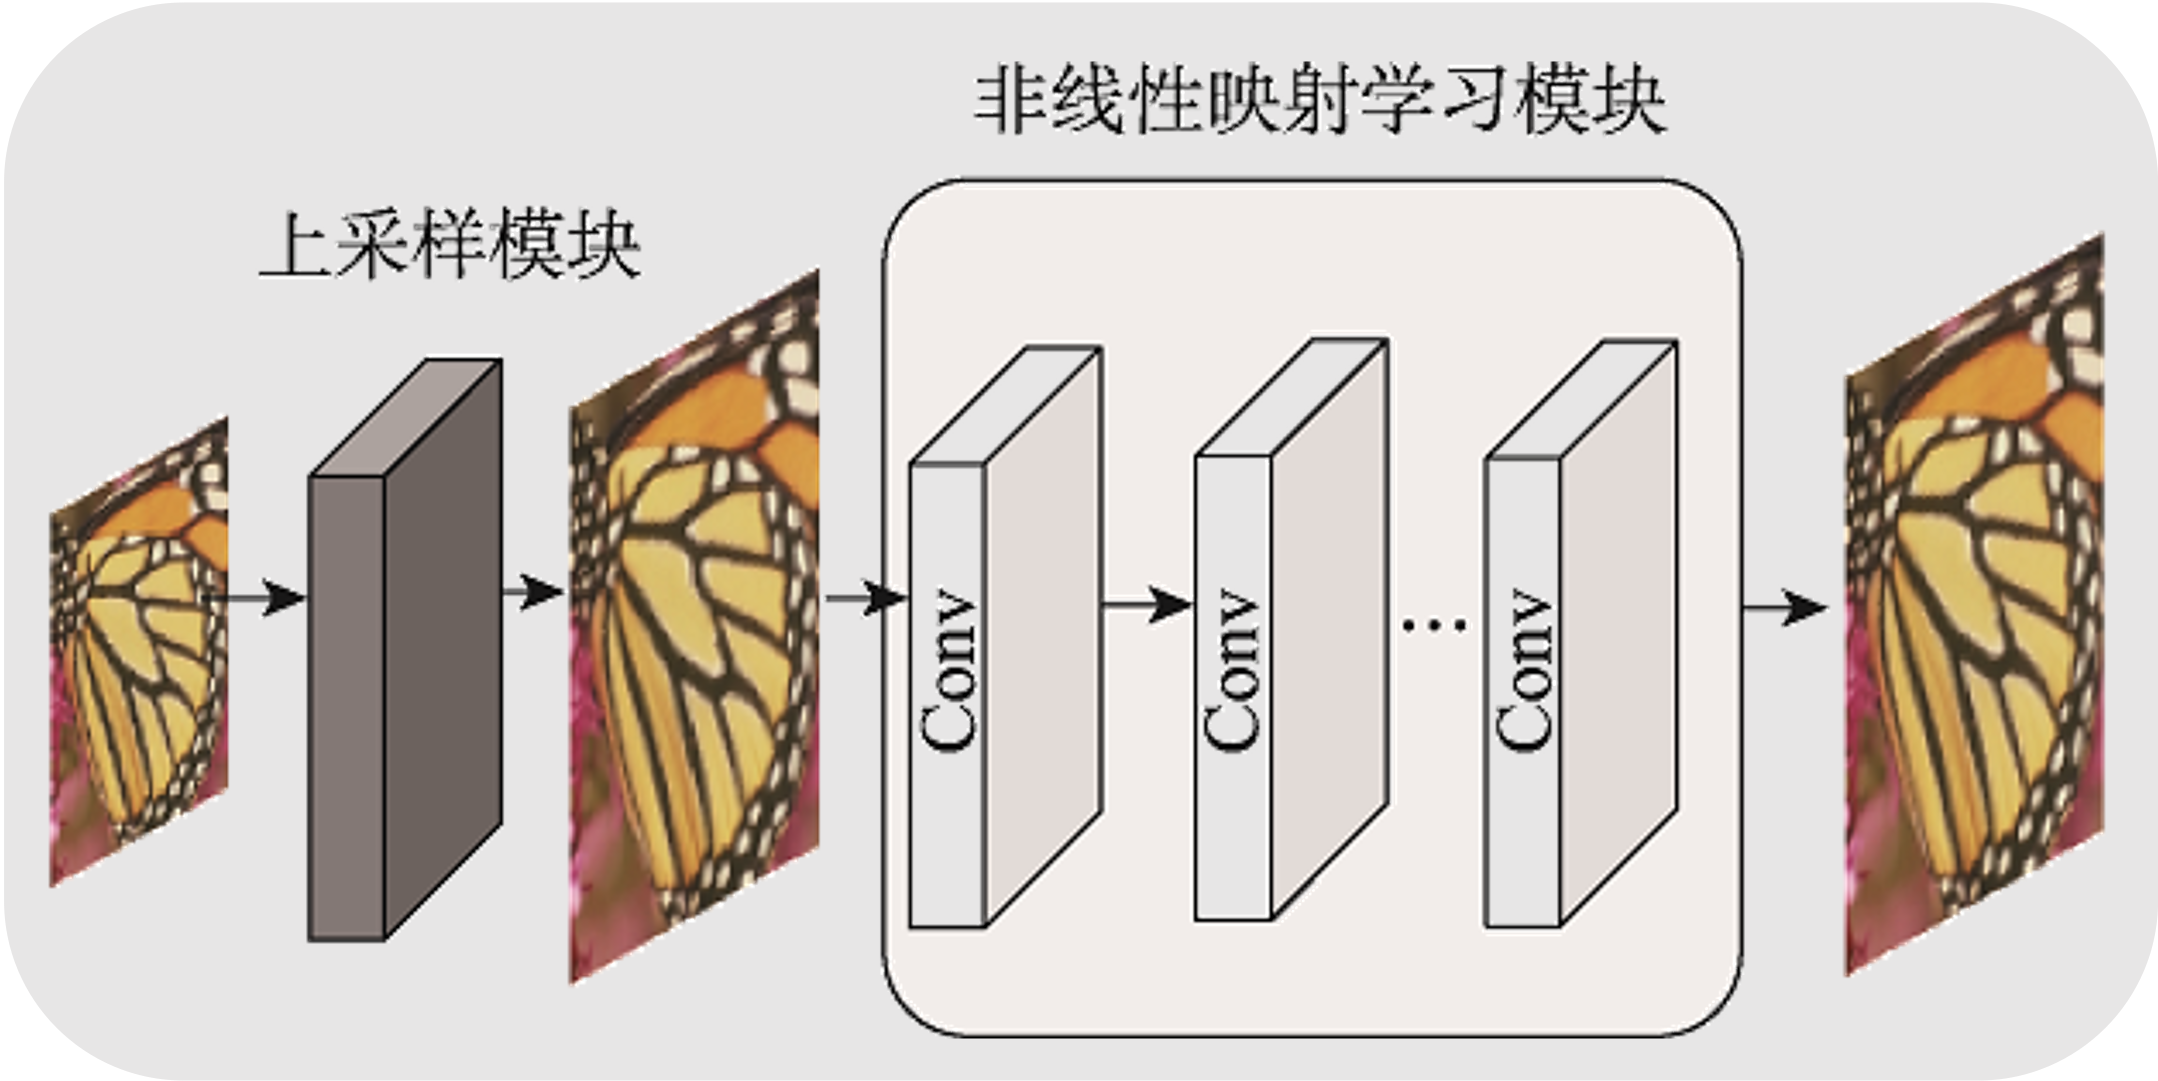
\includegraphics[width=\linewidth]{13-1.png}
     \end{minipage}
  }
   \subfloat[]{
    \begin{minipage}[b]{0.24\linewidth}
      \centering
      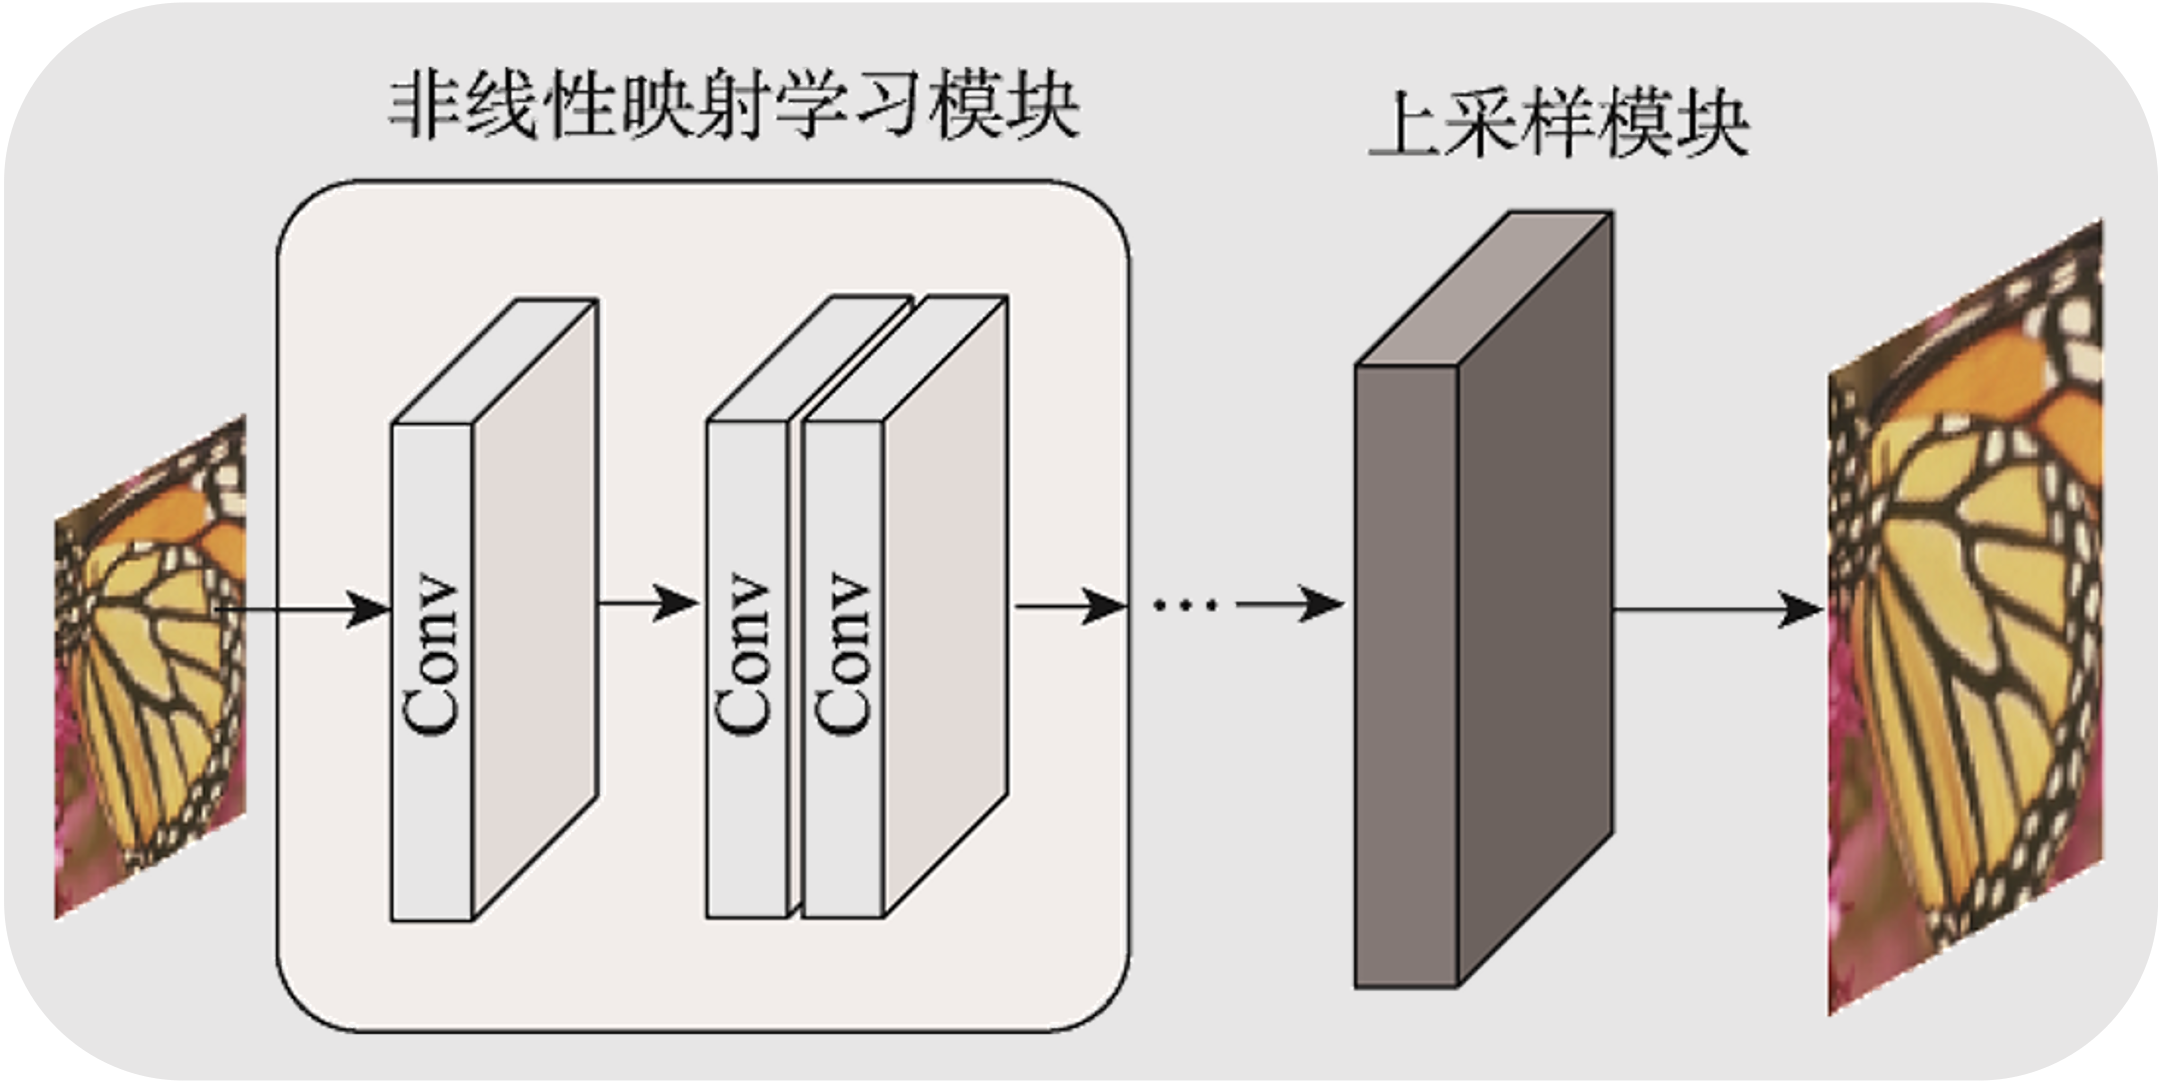
\includegraphics[width=\linewidth]{13-2.png}
     \end{minipage}
  }
  \subfloat[]{
    \begin{minipage}[b]{0.24\linewidth}
      \centering
      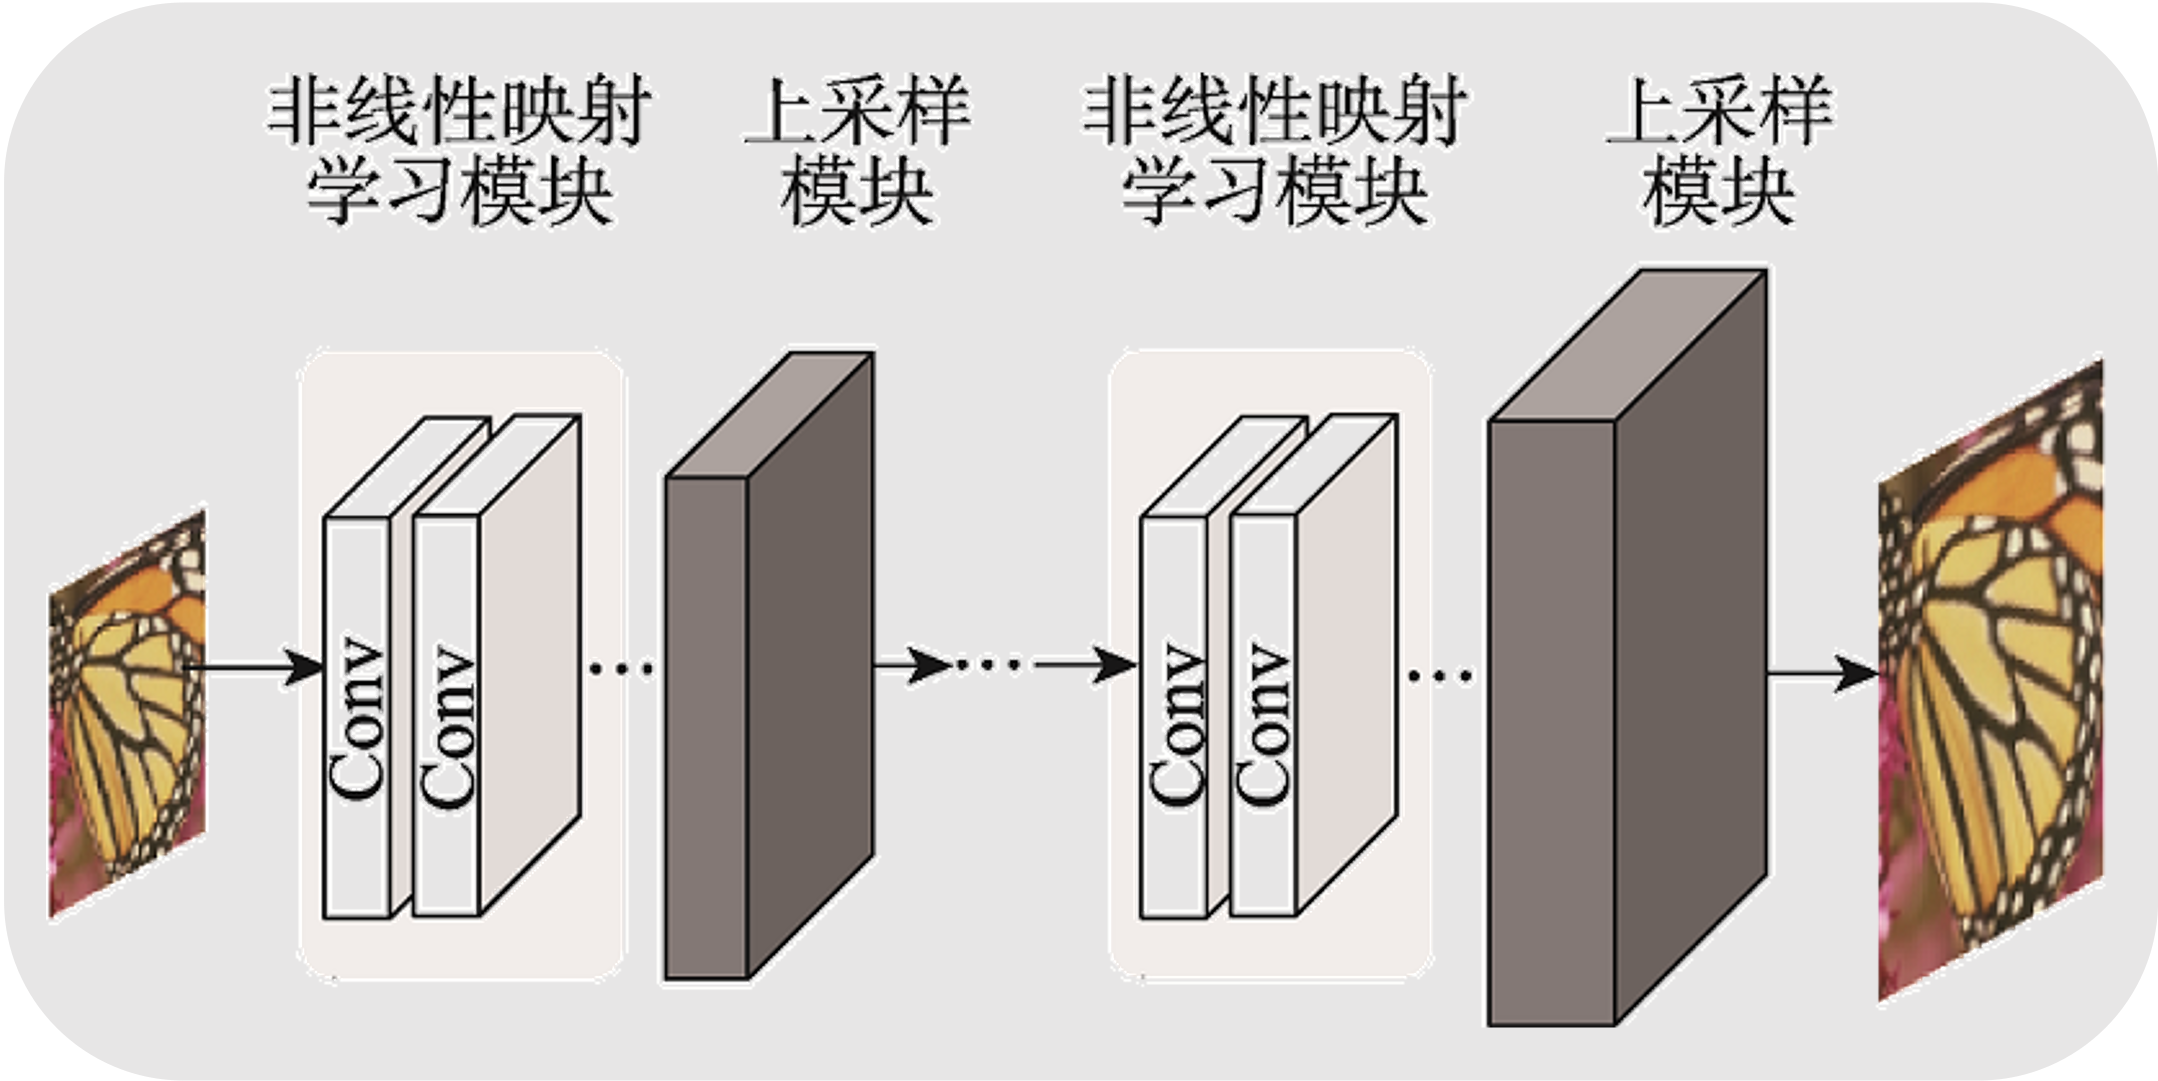
\includegraphics[width=\linewidth]{13-3.png}
     \end{minipage}
  }
   \subfloat[]{
    \begin{minipage}[b]{0.24\linewidth}
      \centering
      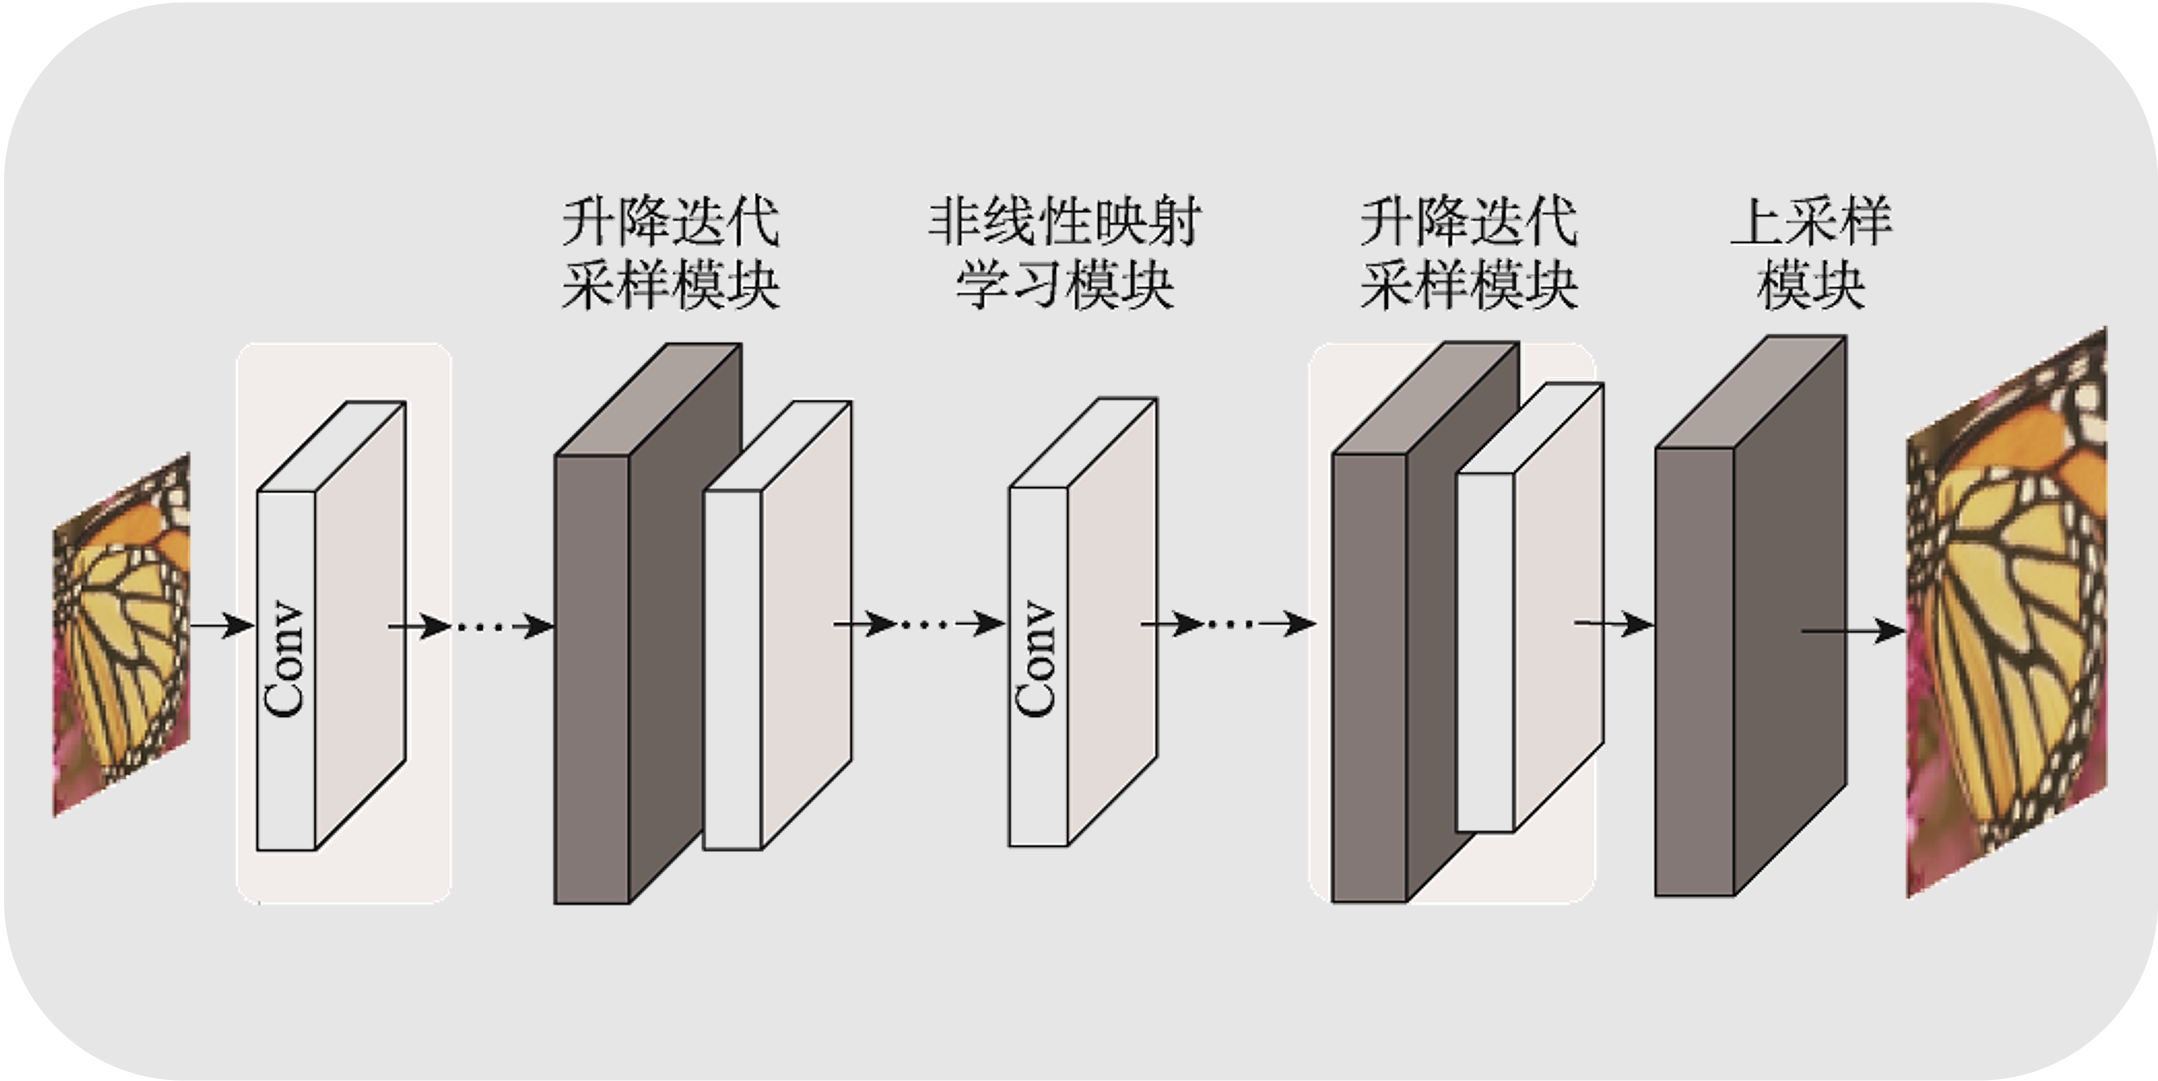
\includegraphics[width=\linewidth]{13-4.png}
     \end{minipage}
  }
    \end{minipage}
  \caption{上采样模块位置不同的超分网络框架:(a) 前端上采样框架;(b) 后端上采样框架;(c) 渐进式上采样框架;(d) 升降采样迭代式框架}
  \label{fig:fig13}
\end{figure*}

SISR 方法的框架由两部分构成,分别是非线性映射学习模块和实现图像放大的上采样模块。非线 性映射学习模块负责完成低分辨率图像到高分辨率 图像的映射,这个过程中利用损失函数来进行引导 和监督学习的进程;上采样模块实现重建图像的放大。两个模块共同协作,最终完成输入图像的超分辨 率重建。根据上采样模块的位置不同,可以将SISR方 法总结为如 \textbf{图 \ref{fig:fig13}} 所示四种超分框架:

\begin{itemize}
	\item \textbf{前端上采样超分框架}可以避免在低维空间上 进行低维到高维的映射学习,降低了学习难度,是一 种简单易行的方法。但是同时噪声和模糊等也被增 强,并且在高维空间进行卷积运算将会增加模型计 算量,消耗更多的计算资源。
	\item \textbf{后端上采样超分框架}针对前端 上采样超分框架存在的问题,提高计算资源利用效 率,研究者提出了后端上采样超分框架,将上采样模 块放置在网络后面部分。该框架下的大部分卷积计算在低维空间进行,最后再利用端到端可学习的上 采样层,如转置卷积和亚像素卷积,进行上采样 放大。这样的好处是进一步释放了卷积的计算能力, 降低模型复杂度。
	\item \textbf{渐进式上采样超分框架}中,图像放大是逐级进行的,中途生成的图像继续输入后续模块,直到达到 目标分辨率。常用方法是采用卷积级联或者 Laplace 金字塔的方式,再结合多级监督等学习策略,就能完 成大的超分倍增系数下的超分重建任务。
	\item \textbf{升降采样迭代式超分框架}借 鉴了反向投影的思想,交替使用上、下采样,结合得到的所有特征图来完成 低分辨率图像的重建。这种方法通过反复进行 LR- HR 的映射学习,能充分学习出两者之间的映射关 系。
\end{itemize}

\begin{figure}[!t]
	\centering
	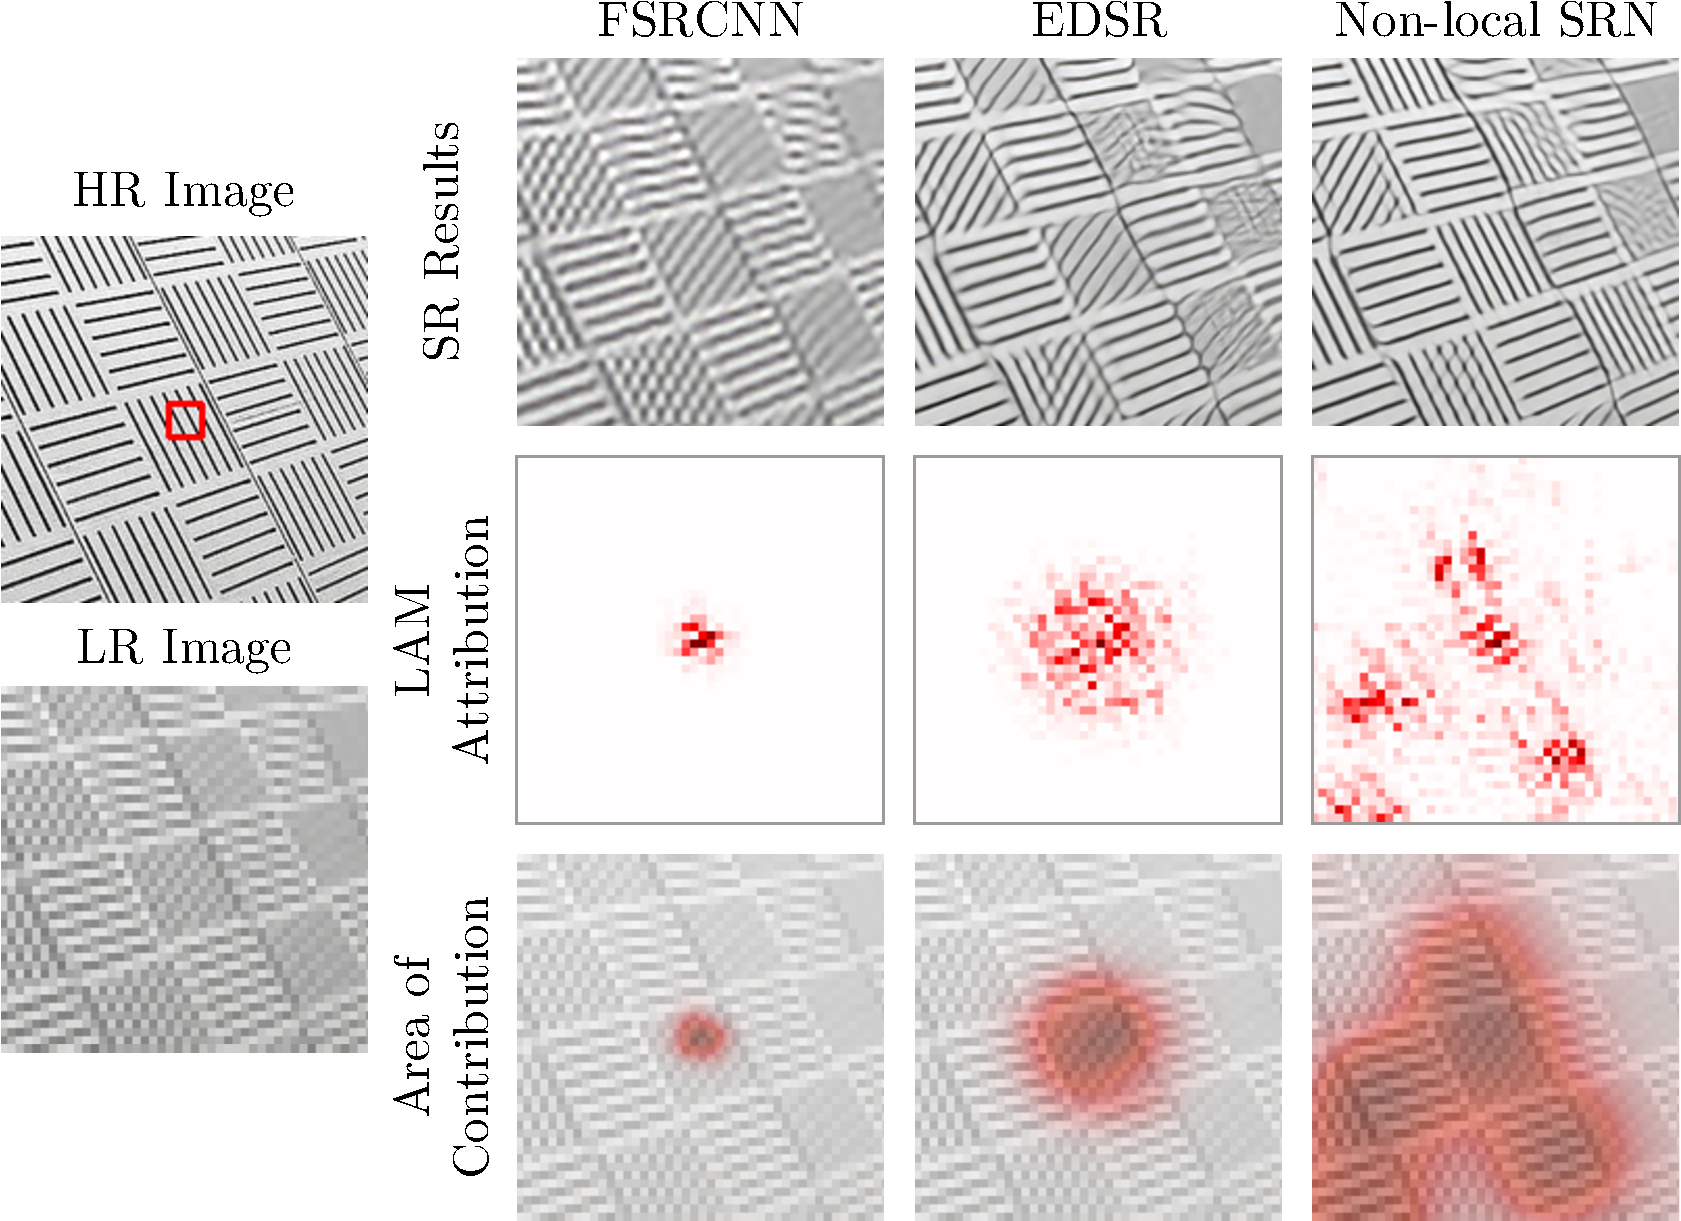
\includegraphics[width=\linewidth]{10}
	\caption{用于图像超分辨率重建网络解释的局部归因图(LAM Attribution, LAM)方法的可视化结果。LAM 图表示输入 LR 图像中每个像素的重要性}
	\label{fig:fig10}
\end{figure}

传统的基于卷积神经网络的图像超分辨率重建方法,为了建立 LR 图像和 HR 图像的映射关系并能恢复图像更加精细的细节,大多从模型的骨干网络(如 VGG、ResNet),上采样方法(如反卷积、亚像素层),多尺度策略(如特征金字塔、密集连接),注意力机制(如通道注意力和空间注意力)等来充分地利用低分辨率图像的先验信息,重建出缺失的高频信息。除了对网络架构和模块设计的研究, Dong 等 \cite{DBLP:conf/cvpr/GuD21}从超分网络可解释性的角度对图像重建进行研究,利用局部归因局部归因图的方法对超分结果进行归因分析。如 \textbf{图 \ref{fig:fig10}} 是一张 LR 图通过不同的模型超分成一张 SR 图的结果。HR 图上有一个红色的框,LAM Attribution 就代表了三个不同的超分模型输入的 LR 图像中每个像素对红色的框 SR 结果的重要性。对 HR 图像中间红框处的超分结果进行归因分析,右边图像上标红的像素即为对该超分结果``贡献比较大''的像素。LAM 结果表明,FSRCNN 仅利用非常有限的信息,EDSR 增加了信息利用的范围,但仍然无法重建精确的纹理,而非局部网络 RNAN 可以利用更大范围的信息来获得更好的超分结果。

\begin{figure*}[!htbp]
	\centering
	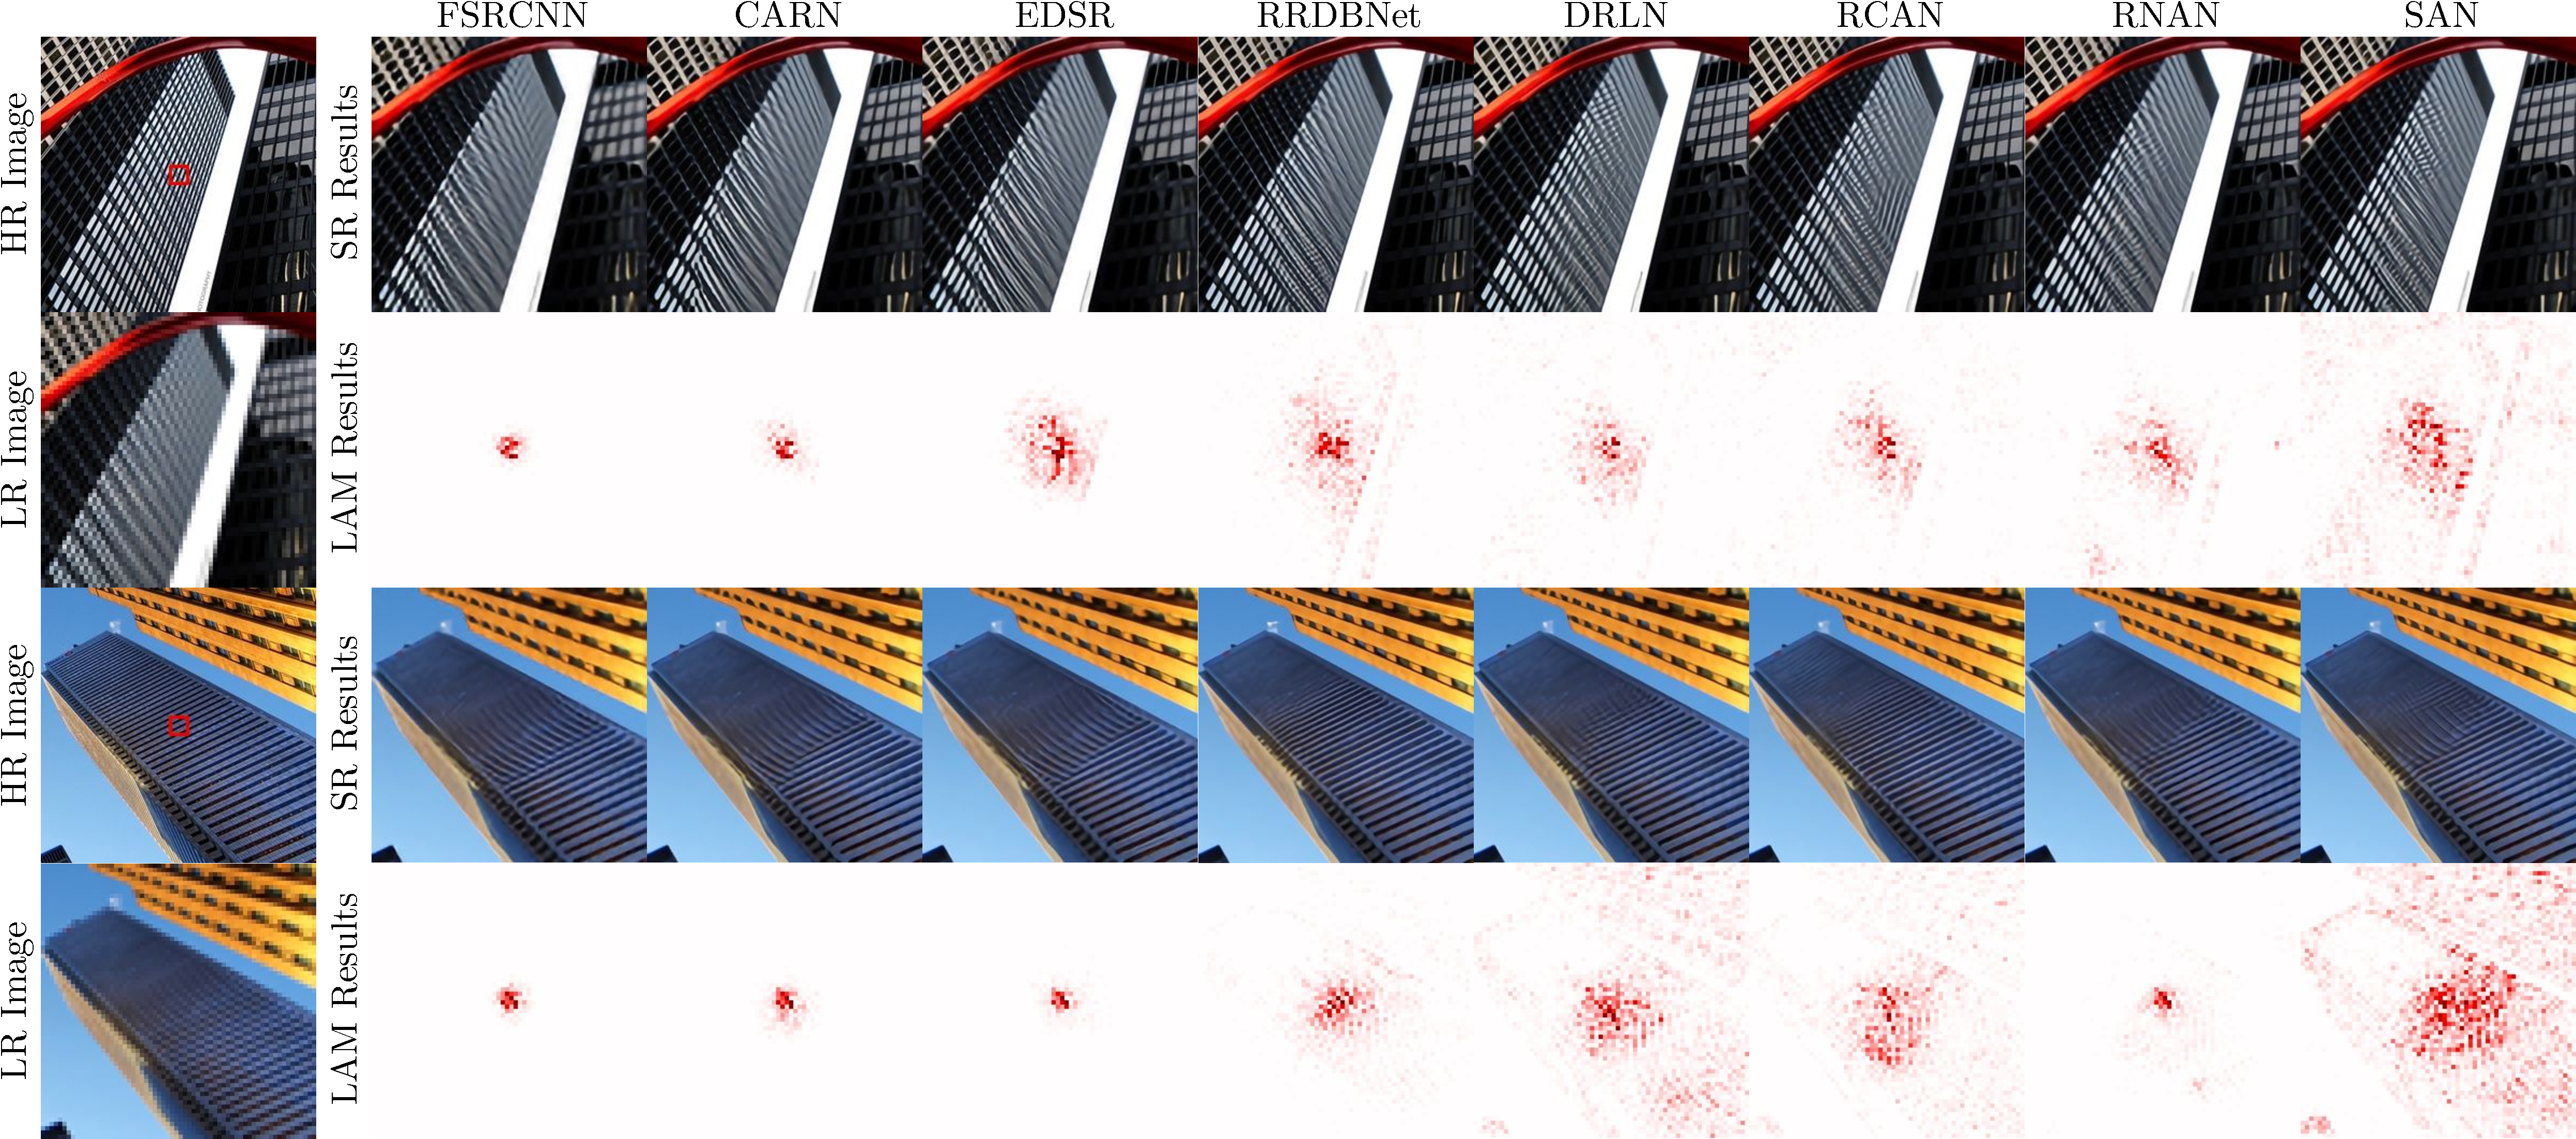
\includegraphics[width=\linewidth]{11}
	\caption{LAM 实验结果}
	\label{fig:fig11}
\end{figure*}

不同 SR 模型的 LAM 结果如 \textbf{图 \ref{fig:fig11}} 所示。有以下的观察:

\begin{enumerate}
	\item 早期的网络 FSRCNN 和浅层网络 CARN 的归因图有效区域相对较小,意味着这些模型只能基于有限的周围像素进行超分。
	\item 深度残差网络,即 EDSR,RRDBNet,RCAN 和 DRLN,具有更深的架构和更大的归因图有效区域。这些网络对 LR 图像中具有相似图案的更大范围的像素感兴趣,例如,摩天大楼上出现的规则条纹。尽管这些区域中的纹理在 LR 图像中严重混叠,这可能误导 SR 过程,但是一些网络仍然重建精确的纹理,并且根据 LAM 结果,它们注意到更大范围的未混叠区域。
	\item 对于有 non-local 和 channel-wise attention 模块的超分模型,它们会利用更长距离的信息来协助 SR 的过程。代表性模型包括 RNAN,RNAN 和 SAN。
\end{enumerate}

受 Transformer 在诸多计算机视觉任务上取得优异表现的驱动,越来越多的研究也将其引入到图像超分辨率重建任务中,并一度刷新图像超分辨率重建的性能。显然,这得益于 Transformer 对远程依赖建模的能力,使得他相比较于卷积神经网络模型可以看到更多的像素。但 Dong 等人 \cite{DBLP:journals/corr/abs-2205-04437}利用局部归因图研究发现对于 CNN-based methods 例如 RCAN,EDSR 这一想法是正确的。然而对于 Transformer-based method SwinIR 来讲,LAM 的结果并没有表明 SwinIR 比 RCAN 利用的信息多。说明 SwinIR 比 CNN 有更强的映射能力,能利用更少的信息获得更好的效果。其次,SwinIR 在 exploit input pixels 仍有提升空间。基于此,他们设计了 Hybrid Attention Transformer 来结合 channel attention 和 self-attention 两种方案,以利用前者对全局信息的利用能力和后者强大的表示能力。 此外,为了更好地聚合跨窗口信息,引入了一个重叠的交叉注意模块。实验结果如 \textbf{表 \ref{quantitative results}} 所示,可以看到, Transformer-based method 几乎已经成为图像超分辨率重建任务的主流研究框架。

如 \textbf{图 \ref{fig:fig12}} 所示的热图展示了不同 SR 网络的关注区域,所有的 SR 网络都关注红色的区域,不同 SR 模型关注区域的不同体现在蓝色区域上。 如何提取和利用蓝色区域的信息是一个 SR 网络区别于其他网络的关键因素。在图6的第6、第7和第8个例子中,SR 网络的注意力沿着纹理延伸的方向分布;在第9个例子中,SR 网络注意到目标补丁周围形状相似的窗口。

\begin{figure*}[!htbp]
	\centering
	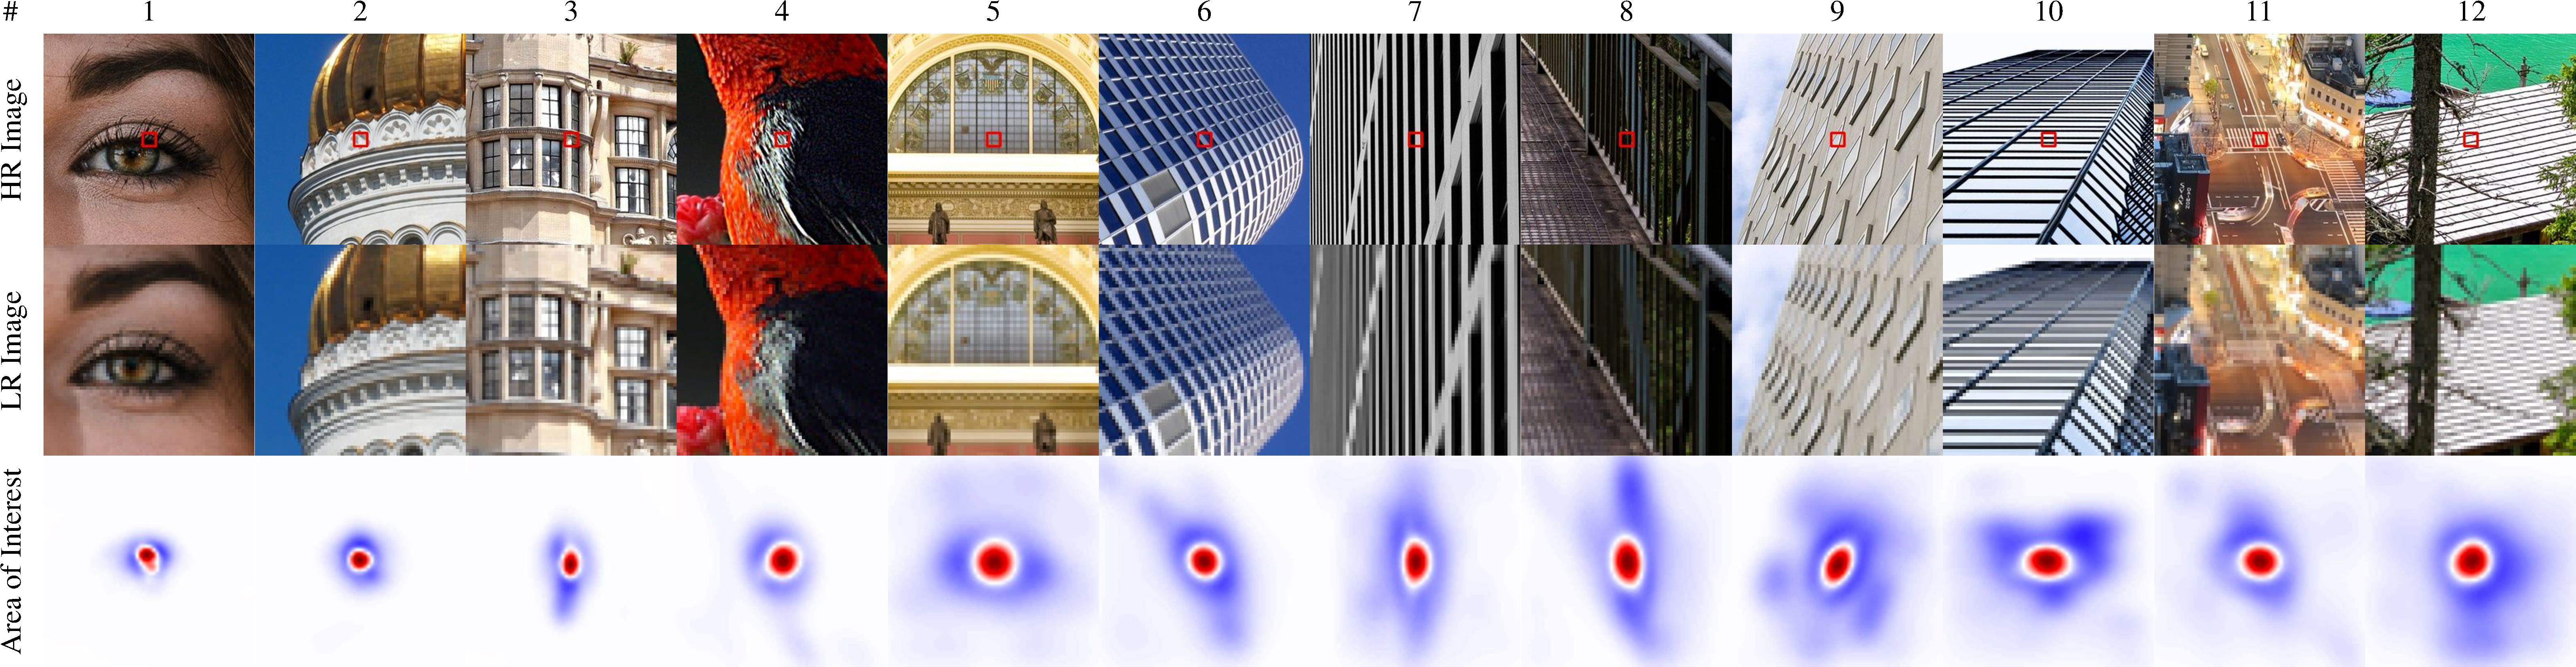
\includegraphics[width=\linewidth]{12}
	\caption{热图展示了不同 SR 网络的关注区域,所有 SR 网络都关注红色的区域,不同 SR 模型关注区域的不同体现在蓝色区域}
	\label{fig:fig12}
\end{figure*}


\begin{table*}[!htbp]
\scriptsize
\center
\begin{center}
\caption{在基准数据集上与 SOTA 的方法进行定量比较。前三的方法用 \textcolor{red}{红色}, \textcolor{blue}{蓝色} 和~  {\color[HTML]{00BF01} 绿色} 标注。 ``$\dagger$'' 表示该方法在 ImageNet 上进行预训练}
\label{quantitative results}
\begin{adjustbox}{width=\linewidth}
\renewcommand{\arraystretch}{1.3}
% \linespread{1.3}
% \vspace{2mm}
%\resizebox{\textwidth}{70mm}{
\begin{tabular}{|l|c|c|c|c|c|c|c|c|c|c|c|c|}
\hline
\multirow{2}{*}{Method} & \multirow{2}{*}{Scale} & \multirow{2}{*}{\makecell{Training\\Dataset}} &
\multicolumn{2}{c|}{Set5~\cite{DBLP:conf/bmvc/BevilacquaRGA12}} &  \multicolumn{2}{c|}{Set14~\cite{DBLP:conf/cas/ZeydeEP10}} &  \multicolumn{2}{c|}{BSD100~\cite{DBLP:conf/iccv/MartinFTM01}} &  \multicolumn{2}{c|}{Urban100~\cite{DBLP:conf/cvpr/HuangSA15}} &  \multicolumn{2}{c|}{Manga109~\cite{DBLP:journals/mta/MatsuiIAFOYA17}}  
\\ 
%\hline
\cline{4-13}
&  &  & PSNR & SSIM & PSNR & SSIM & PSNR & SSIM & PSNR & SSIM & PSNR & SSIM 
\\ 
\hline
\hline
EDSR~\cite{DBLP:conf/cvpr/LimSKNL17} & $\times$2 & DIV2K %
& 38.11
& 0.9602
& 33.92
& 0.9195
& 32.32
& 0.9013
& 32.93
& 0.9351
& 39.10
& 0.9773
\\
RCAN~\cite{DBLP:journals/corr/abs-2201-11279} & $\times$2 & DIV2K %
& 38.27
& 0.9614
& 34.12
& 0.9216
& 32.41
& 0.9027
& 33.34
& 0.9384
& 39.44
& 0.9786
\\  
SAN~\cite{DBLP:conf/cvpr/DaiCZXZ19} & $\times$2 & DIV2K %
& {38.31}
& {0.9620}
& {34.07}
& {0.9213}
& {32.42}
& {0.9028}
& {33.10}
& {0.9370}
& {39.32}
& {0.9792}\\
IGNN~\cite{zhou2020cross} & $\times$2 & DIV2K %
& {38.24}
& {0.9613}
& {34.07}
& {0.9217}
& {32.41}
& {0.9025}
& {33.23}
& {0.9383}
& {39.35}
& {0.9786}
\\
HAN~\cite{niu2020single} & $\times$2 & DIV2K %
& {38.27}
& {0.9614}
& {34.16}
& {0.9217}
& {32.41}
& {0.9027}
& {33.35}
& {0.9385}
& {39.46}
& {0.9785}              
\\
NLSN~\cite{mei2021image} & $\times$2 & DIV2K %
& 38.34 
& 0.9618 
& 34.08 
& 0.9231
& 32.43 
& 0.9027 
& 33.42
& 0.9394
& 39.59
& 0.9789
\\
RCAN-it~\cite{DBLP:journals/corr/abs-2201-11279} & $\times$2 & DF2K %
& 38.37
& 0.9620
& 34.49
& 0.9250
& 32.48
& 0.9034
& 33.62
& 0.9410
& 39.88
& 0.9799
\\
SwinIR~\cite{DBLP:conf/iccvw/LiangCSZGT21} & $\times$2 & DF2K %
& 38.42
& 0.9623
& 34.46
& 0.9250
& 32.53
& 0.9041
& 33.81
& 0.9427
& 39.92
& 0.9797
\\
EDT~\cite{DBLP:journals/corr/abs-2112-10175} & $\times$2 & DF2K %
& 38.45
& 0.9624
& 34.57
& 0.9258
& 32.52
& 0.9041
& 33.80
& 0.9425
& 39.93
& 0.9800
\\
\textbf{HAT} (ours) & $\times$2 & DF2K %
& {\color[HTML]{00BF01} 38.63}
& {0.9630}
& {\color[HTML]{00BF01} 34.86}
& {\color[HTML]{00BF01} 0.9274}
& {\color[HTML]{00BF01} 32.62}
& {\color[HTML]{00BF01} 0.9053}
& {\color[HTML]{00BF01} 34.45}
& {\color[HTML]{00BF01} 0.9466}
& {40.26}
& {0.9809}
\\
\hdashline
IPT$^\dagger$~\cite{DBLP:conf/cvpr/Chen000DLMX0021} & $\times$2 & ImageNet %
& {38.37}
& {-}
& {34.43}
& {-}
& {32.48}
& {-}
& {33.76}
& {-}
& {-}
& {-}
\\
EDT$^\dagger$~\cite{DBLP:journals/corr/abs-2112-10175} & $\times$2 & DF2K %
& {\color[HTML]{00BF01} 38.63}
& {\color[HTML]{00BF01} 0.9632}
& 34.80
& 0.9273
& {\color[HTML]{00BF01} 32.62}
& {0.9052}
& 34.27
& 0.9456
& {\color[HTML]{00BF01} 40.37}
& {\color[HTML]{00BF01} 0.9811}
\\
\textbf{HAT}$^\dagger$ (ours) & $\times$2 & DF2K %
& \textcolor{blue}{38.73}
& \textcolor{blue}{0.9637}
& \textcolor{blue}{35.13}
& \textcolor{blue}{0.9282}
& \textcolor{blue}{32.69}
& \textcolor{blue}{0.9060}
& \textcolor{blue}{34.81}
& \textcolor{blue}{0.9489}
& \textcolor{blue}{40.71}
& \textcolor{blue}{0.9819}
\\
\textbf{HAT-L}$^\dagger$ (ours) & $\times$2 & DF2K %
& \textcolor{red}{38.91}
& \textcolor{red}{0.9646}
& \textcolor{red}{35.29}
& \textcolor{red}{0.9293}
& \textcolor{red}{32.74}
& \textcolor{red}{0.9066}
& \textcolor{red}{35.09}
& \textcolor{red}{0.9505}
& \textcolor{red}{41.01}
& \textcolor{red}{0.9831}
\\
\hline
\hline
EDSR~\cite{DBLP:conf/cvpr/LimSKNL17} & $\times$3 & DIV2K %
& 34.65
& 0.9280
& 30.52
& 0.8462
& 29.25
& 0.8093
& 28.80
& 0.8653
& 34.17
& 0.9476
\\
RCAN~\cite{DBLP:journals/corr/abs-2201-11279} & $\times$3 & DIV2K %
& 34.74
& 0.9299
& 30.65
& 0.8482
& 29.32
& 0.8111
& 29.09
& 0.8702
& 34.44
& 0.9499
\\
SAN~\cite{DBLP:conf/cvpr/DaiCZXZ19} & $\times$3 & DIV2K %
& {34.75}
& {0.9300}
& {30.59}
& {0.8476}
& {29.33}
& {0.8112}
& {28.93}
& {0.8671}
& {34.30}
& {0.9494}
\\
IGNN~\cite{zhou2020cross} & $\times$3 & DIV2K %
& {34.72}
& {0.9298}
& {30.66}
& {0.8484}
& {29.31}
& {0.8105}
& {29.03}
& {0.8696}
& {34.39}
& {0.9496}
\\
HAN~\cite{niu2020single}  & $\times$3 & DIV2K %
& {34.75}
& {0.9299}
& {30.67}
& {0.8483}
& {29.32}
& {0.8110}
& {29.10}
& {0.8705}
& {34.48}
& {0.9500}
\\
NLSN~\cite{mei2021image} & $\times$3 & DIV2K %
& 34.85 
& 0.9306 
& 30.70 
& 0.8485 
& 29.34 
& 0.8117 
& {29.25}
& {0.8726}
& 34.57 
& 0.9508  
\\
RCAN-it~\cite{DBLP:journals/corr/abs-2201-11279} & $\times$3 & DF2K %
& {34.86}
& {0.9308}
& {30.76}
& {0.8505}
& {29.39}
& {0.8125}
& {29.38}
& {0.8755}
& {34.92}
& {0.9520}
\\
SwinIR~\cite{DBLP:conf/iccvw/LiangCSZGT21} & $\times$3 & DF2K %
& 34.97
& 0.9318
& 30.93
& 0.8534
& 29.46
& 0.8145
& 29.75
& 0.8826
& 35.12
& 0.9537
\\
EDT~\cite{DBLP:journals/corr/abs-2112-10175} & $\times$3 & DF2K %
& 34.97
& 0.9316
& 30.89
& 0.8527
& 29.44
& 0.8142
& 29.72
& 0.8814
& 35.13
& 0.9534
\\
\textbf{HAT} (ours) & $\times$3 & DF2K %
& {35.06}
& {\color[HTML]{00BF01} 0.9329}
& {31.08}
& {\color[HTML]{00BF01} 0.8555}
& {\color[HTML]{00BF01} 29.54}
& {\color[HTML]{00BF01} 0.8167}
& {\color[HTML]{00BF01} 30.23}
& {\color[HTML]{00BF01} 0.8896}
& {\color[HTML]{00BF01} 35.53}
& {\color[HTML]{00BF01} 0.9552}
\\
\hdashline
IPT$^\dagger$~\cite{DBLP:conf/cvpr/Chen000DLMX0021} & $\times$3 & ImageNet %
& {34.81}
& {-}
& {30.85}
& {-}
& {29.38}
& {-}
& {29.49}
& {-}
& {-}
& {-}
\\
EDT$^\dagger$~\cite{DBLP:journals/corr/abs-2112-10175} & $\times$3 & DF2K %
& {\color[HTML]{00BF01} 35.13}
& 0.9328
& {\color[HTML]{00BF01} 31.09}
& 0.8553
& {29.53}
& {0.8165}
& 30.07
& 0.8863
& 35.47
& 0.9550
\\
\textbf{HAT}$^\dagger$ (ours) & $\times$3 & DF2K %
& \textcolor{blue}{35.16}
& \textcolor{blue}{0.9335}
& \textcolor{blue}{31.33}
& \textcolor{blue}{0.8576}
& \textcolor{blue}{29.59}
& \textcolor{blue}{0.8177}
& \textcolor{blue}{30.70}
& \textcolor{blue}{0.8949}
& \textcolor{blue}{35.84}
& \textcolor{blue}{0.9567}
\\
\textbf{HAT-L}$^\dagger$ (ours) & $\times$3 & DF2K %
& \textcolor{red}{35.28}
& \textcolor{red}{0.9345}
& \textcolor{red}{31.47}
& \textcolor{red}{0.8584}
& \textcolor{red}{29.63}
& \textcolor{red}{0.8191}
& \textcolor{red}{30.92}
& \textcolor{red}{0.8981}
& \textcolor{red}{36.02}
& \textcolor{red}{0.9576}
\\
\hline
\hline
EDSR~\cite{DBLP:conf/cvpr/LimSKNL17} & $\times$4 & DIV2K %
& 32.46
& 0.8968
& 28.80
& 0.7876
& 27.71
& 0.7420
& 26.64
& 0.8033
& 31.02
& 0.9148
\\
RCAN~\cite{DBLP:journals/corr/abs-2201-11279} & $\times$4 & DIV2K %
& 32.63
& 0.9002
& 28.87
& 0.7889
& 27.77
& 0.7436
& 26.82
& 0.8087
& 31.22
& 0.9173
\\
SAN~\cite{DBLP:conf/cvpr/DaiCZXZ19} & $\times$4 & DIV2K %
& {32.64}
& {0.9003}
& {28.92}
& {0.7888}
& {27.78}
& {0.7436}
& {26.79}
& {0.8068}
& {31.18}
& {0.9169}
\\
IGNN~\cite{zhou2020cross} & $\times$4 & DIV2K %
& {32.57}
& {0.8998}
& {28.85}
& {0.7891}
& {27.77}
& {0.7434}
& {26.84}
& {0.8090}
& {31.28}
& {0.9182}
\\
HAN~\cite{niu2020single} & $\times$4 & DIV2K %
& {32.64}
& {0.9002}
& {28.90}
& {0.7890}
& {27.80}
& {0.7442}
& {26.85}
& {0.8094}
& {31.42}
& {0.9177}
\\
NLSN~\cite{mei2021image} & $\times$4 & DIV2K %
& 32.59 
& 0.9000 
& 28.87 
& 0.7891 
& 27.78 
& 0.7444 
& {26.96}
& {0.8109}
& 31.27 
& 0.9184
\\
RRDB~\cite{DBLP:conf/iccvw/WangXDS21} & $\times$4 & DF2K %
& {32.73}
& {0.9011 }
& {28.99}
& {0.7917}
& {27.85}
& {0.7455}
& {27.03}
& {0.8153}
& {31.66}
& {0.9196}
\\
RCAN-it~\cite{DBLP:journals/corr/abs-2201-11279} & $\times$4 & DF2K %
& 32.69
& 0.9007
& 28.99
& 0.7922
& 27.87
& 0.7459
& 27.16
& 0.8168
& 31.78
& 0.9217
\\
SwinIR~\cite{DBLP:conf/iccvw/LiangCSZGT21} & $\times$4 & DF2K %
& 32.92
& 0.9044
& 29.09
& 0.7950
& 27.92
& 0.7489
& 27.45
& 0.8254
& 32.03
& 0.9260
\\
EDT~\cite{DBLP:journals/corr/abs-2112-10175} & $\times$4 & DF2K %
& 32.82
& 0.9031
& 29.09
& 0.7939
& 27.91
& 0.7483
& 27.46
& 0.8246
& 32.05
& 0.9254
\\
\textbf{HAT} (ours) & $\times$4 & DF2K %
& {33.04}
& {\color[HTML]{00BF01} 0.9056}
& {\color[HTML]{00BF01} 29.23}
& {\color[HTML]{00BF01} 0.7973}
& {\color[HTML]{00BF01} 28.00}
& {\color[HTML]{00BF01} 0.7517}
& {\color[HTML]{00BF01} 27.97}
& {\color[HTML]{00BF01} 0.8368}
& {\color[HTML]{00BF01} 32.48}
& {\color[HTML]{00BF01} 0.9292}
\\
\hdashline
IPT$^\dagger$~\cite{DBLP:conf/cvpr/Chen000DLMX0021} & $\times$4 & ImageNet %
& {32.64}
& {-}
& {29.01}
& {-}
& {27.82}
& {-}
& {27.26}
& {-}
& {-}
& {-}
\\
EDT$^\dagger$~\cite{DBLP:journals/corr/abs-2112-10175} & $\times$4 & DF2K %
& {\color[HTML]{00BF01} 33.06}
& {0.9055}
& {\color[HTML]{00BF01} 29.23}
& {0.7971}
& {27.99}
& 0.7510
& 27.75
& 0.8317
& 32.39
& 0.9283
\\
\textbf{HAT}$^\dagger$ (ours) & $\times$4 & DF2K %
& \textcolor{blue}{33.18}
& \textcolor{blue}{0.9073}
& \textcolor{blue}{29.38}
& \textcolor{blue}{0.8001}
& \textcolor{blue}{28.05}
& \textcolor{blue}{0.7534}
& \textcolor{blue}{28.37}
& \textcolor{blue}{0.8447}
& \textcolor{blue}{32.87}
& \textcolor{blue}{0.9319}
\\
\textbf{HAT-L}$^\dagger$ (ours) & $\times$4 & DF2K %
& \textcolor{red}{33.30}
& \textcolor{red}{0.9083}
& \textcolor{red}{29.47}
& \textcolor{red}{0.8015}
& \textcolor{red}{28.09}
& \textcolor{red}{0.7551}
& \textcolor{red}{28.60}
& \textcolor{red}{0.8498}
& \textcolor{red}{33.09}
& \textcolor{red}{0.9335}
\\
\hline             
\end{tabular}
\end{adjustbox}
%}
\end{center}
\end{table*}


\section{图像分析}
\label{sec:image_analysis}

对图像进行增强、恢复、编码等处理时,输入是 图像,所要求的输出是一幅近似于输入的图像, 这是此类处理的特点。图像处理的另一主要分支 是图像分析,这类处理的输入仍然是图像,但所 要求的输出是对已知图像的描述。分析一般针对图像中的特定区域或目标。为此,传 统算法首先要进行分割(检测),有些分割运算可直接用于整个图像,而有些分割算法只适用于已被 局部分割的图像。传统图像分割是指根据灰度、彩色、空间纹理、几何形状等特征把图像划分成若干个互不相交的区域,使得这些特征在同一区域内表现出一致性或相似性,而在不同区域间表现出明显的不同。简单的说就是在一副图像中,把目标从背景中分离出来。

早期的图像分割主要是通过提取图像手工设计的特征,然后进行分割,分割出来的结果并没有语义的标注,换句话说,分割出来的东西并不知道是什么。随着计算机能力的提高,人们开始考虑获得图像的语义分割,这里的语义主要指分割出来的物体的类别。随着FCN的出现,深度学习正式进入图像语义分割领域,这里的语义仍主要指分割出来的物体的类别,从分割结果可以清楚的知道分割出来的是什么物体。而实例分割则可以对同一类别的不同物体进行不同的划分,可以清楚地知道分割出来的左边和右边的两个人不是同一个人。

传统的图像分割方法利用数字图像处理、拓扑学、数学等方面的知识来进行图像分割,比较经典的方法包括灰度阈值分割、样板(模版)匹配和区域生长。本文将主要对灰度阈值分割方法进行探讨。这类方法的核心思想是基于图像的灰度特征来计算一个或多个灰度阈值,并将图像中每个像素的灰度值与阈值相比较,最后将像素根据比较结果分到合适的类别中。因此,该类方法最为关键的一步就是按照某个准则函数来求解最佳的灰度阈值。

基于阈值的分割方法适用于目标和背景占据不同灰度范围的图像。理想情况下,目标和背景在其所属区域内具有恒定的不同灰度,则只需选取一个阈值便可对图像进行分割。但实际上,由于拍摄时的噪声、非均匀照明和目标表面对光照的非均匀反射等因素的干扰,其灰度值并不是恒定的,因此固定阈值分割难以有出色表现。这种情况下,我们可以根据不同图像的特性分别采用不同的阈值进行分割,即自适应阈值分割。

\twocolumn[{%
\renewcommand\twocolumn[1][]{#1}%
\noindent\begin{minipage}{\linewidth} 
 	\begin{center}
 	\captionsetup{font=small}
 	\begin{tabular}{@{}c@{}c@{}c@{}}
 	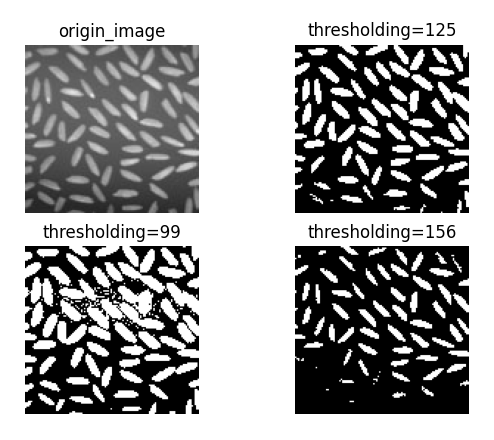
\includegraphics[width=0.31\linewidth,cframe=red!50!black 0.95mm]{14-1} &
 	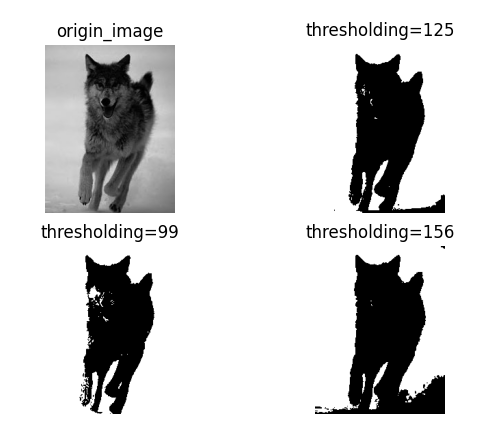
\includegraphics[width=0.31\linewidth,cframe=green!50!black 0.95mm]{14-2} &
    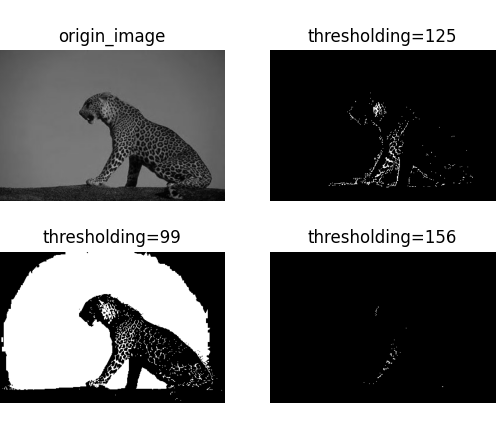
\includegraphics[width=0.313\linewidth,cframe=blue!50!black 0.95mm]{14-3} \vspace{-1mm}\\
%	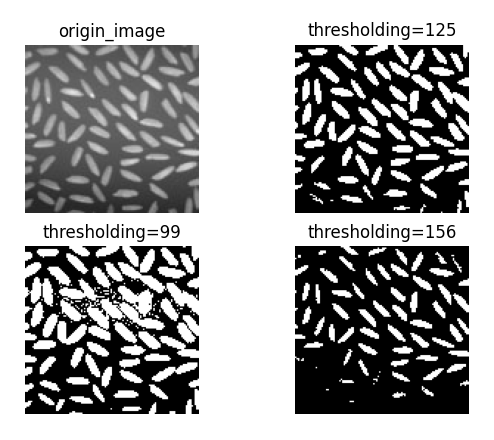
\includegraphics[width=0.31\linewidth]{14-1} &
% 	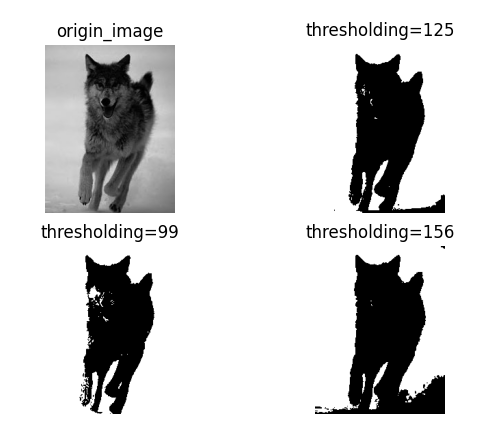
\includegraphics[width=0.31\linewidth]{14-2} &
%    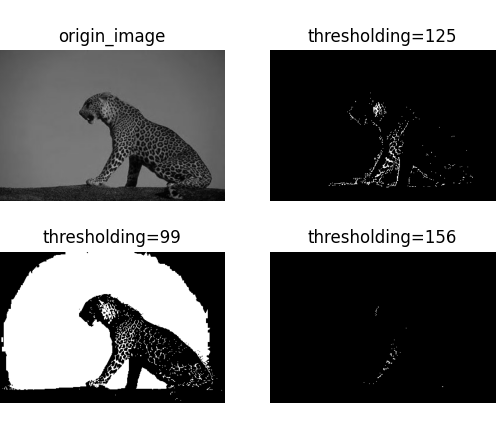
\includegraphics[width=0.32\linewidth]{14-3} \vspace{-1mm}\\
    \end{tabular}
	\captionof{figure}{\small 原始图像及三个不同阈值下的分割结果,三个阈值分别为125(右上)、99(左下)和156(右下)}
	\label{fig:random_thresholding}
	\end{center} 
\end{minipage}
}]

基于阈值的分割方法大多利用了图像的灰度直方图,它很好地反映了一幅图像中的灰度分布信息,是阈值选取的重要参考依据。在对直方图区域进行划分后,可以得到相应的直方图统计信息(目标/背景的先验概率、均值等),由此可以进一步求解不同的阈值选取准则函数。

图像分割旨在根据一定的准则将图像 $I$ 划分为不同区域的集合 $S$,集合 $S$ 满足下列条件:

\begin{enumerate}
	\item $\cup S_i = S$  
	\item $S_i \cap S_j=\emptyset,\;i \neq j$
	\item $\forall S_i,\; P(S_i)=true$
	\item $P(S_i\cup S_j)=false,\; i\neq j,\; S_i \; adjacent \; S_j$
\end{enumerate}
 
对于灰度图像而言,可以将其看作由目标(前景)和背景所构成,基于阈值的分割方法就是通过一个固定阈值将图像中的目标像素与背景像素进行分割,从而实现从图像中提取目标的目的。上述过程可以用下面的公式进行描述:

\begin{equation}
I'(x, y)=\left\{\begin{array}{l}
255, \;I(x, y)>\text{thresholding} \\[2em]
0, \;\quad I(x, y) \leq \text{thresholding}
\end{array}\right.
\vspace{0.5cm}
\end{equation}

其中,$\text{thresholding}$ 是设定的阈值,$x$ 与 $y$ 表示像素在图像中的坐标,$I(x, y)$ 为像素 $(x,y)$ 在原始图像中的灰度值,$I'(x, y)$ 为像素 $(x,y)$ 根据阈值分割后的二值图像对应的像素值。

阈值的选择对于基于阈值的分割方法而言至关重要。在理想条件下,目标和背景的灰度值具有明显的划分,可以将直方图的峰值之间的数值设置为阈值。但在实际应用中,由于各种环境因素的影响,目标和背景的灰度值界限并不易于区分,如 \textbf{图 \ref{fig:random_thresholding}} 所示,阈值设置过低时,背景中的噪声也会被划分到目标类别中,而当阈值设置过高时,目标中灰度值较低的部分被划入了背景部分。此外,对于不同的图像而言,相同的阈值也会取得不同的分割效果。因此,阈值的设置是基于阈值的分割方法的一大难题。图像分割阈值的设置常用方法包括:

\begin{itemize}
	\item 基于直方图形状:对去噪后的直方图的峰值、谷值和曲率等进行分析从而确定阈值
	\item 基于聚类:迭代找到阈值,并基于该阈值进行聚类
	\item 基于熵:选择一个使直方图信息量最大化的阈值
	\item 空间阈值(高阶统计):阈值的选择是基于空间邻域的高阶统计量
	\item 局部阈值:在每个邻域内利用局部统计信息寻找阈值
\end{itemize}

基于直方图的自适应阈值分割方法将图像的灰度直方图中的目标分量和背景分量分别参数化为模型(如高斯分布),然后在图像的灰度范围内迭代地设置不同的阈值,在当前阈值下,可以利用直方图的信息对模型中的未知参数进行估计(如高斯分布的均值、方差等),进而利用估计的参数对图像的整体灰度直方图进行“预测”。在同时具有“预测”分布和真实分布的情况下,就可以对不同阈值下“预测”的模型或分布进行评价,从而获得使拟合效果最好的阈值。

像的灰度直方图可以反映一幅图像中的灰度分布信息,能够为阈值的选取提供重要参考依据。基于直方图的自适应阈值分割方法,首先利用灰度直方图对图像的灰度分布进行统计。为了去除噪声的影响以及便于后续分布的拟合,要对直方图进行预处理,可以采用均值滤波或一维高斯滤波。为了对滤波处理后的灰度分布曲线进行拟合,同时将图像中的目标灰度值与背景灰度值进行区分,就需要分别建立符合目标和背景分量的直方图形状的参数模型,一般假设目标分量和背景分量的直方图形状近似服从高斯分布,而图像整体的灰度直方图形状即为由两个高斯分布组成的混合高斯分布。因此,在基于直方图的自适应阈值分割方法中,用下面两个高斯分布来分别代表目标和背景的分布:

\begin{equation}
f_o(g)=\frac{1}{\sqrt{2 \pi} \sigma_o} e^{-1 / 2\left(\frac{g-\mu_o}{\sigma_o}\right)^2}
\end{equation}

\begin{equation}
f_b(g)=\frac{1}{\sqrt{2 \pi} \sigma_b} e^{-1 / 2\left(\frac{g-\mu_b}{\sigma_b}\right)^2}
\vspace{0.5cm}
\end{equation}

其中,$f_o(g)$ 和 $f_b(g)$ 分别为目标和背景的分布函数,同时也表示灰度值为 $g$ 的像素占图像总体像素的百分比,$\mu_o$ 和 $\mu_b$ 分别为目标和背景的灰度均值,$sigma_o$ 和 $sigma_b$ 分别为目标和背景的标准差。

我们希望阈值可以将目标和背景的灰度分布进行分割,换句话来说,就是目标和背景的灰度可以分别分布在阈值的左右两侧。因此,我们可以假定一个阈值 $t$,然后对灰度图像直方图中阈值 $t$ 左右两侧的灰度信息进行统计计算,从而可以利用统计数据对 $f_o(g)$ 和 $f_b(g)$ 的均值及标准差进行估计,其估计方法如下所示:

\begin{equation}
\mu_o(t)=\sum_{g=0}^t f(g) g \quad \mu_b(t)=\sum_{g=t+1}^{\text {max }} f(g) g
\end{equation}

\begin{equation}
\sigma_o=\sum_{g=0}^t f(g) \left(g-\mu_o\right)  \quad \sigma_b=\sum_{g=t+1}^{\text {max }} f(g) \left(g-\mu_b\right)
\end{equation}

根据先验,我们可以得到一个像素落在目标或落在背景的概率分别为:

\begin{equation}
p_o(t)=\sum_t^{g=0} f(g)
\end{equation}

\begin{equation}
p_b(t)=1-p_o(t)
\vspace{0.5cm}
\end{equation}

对于假定的阈值 $t$,可以通过下面的公式对图像整体的灰度分布进行“预测”,并同样利用一维高斯滤波对估计的分布进行滤波处理:

\begin{equation}
P_t(g)=p_o f_0(g)+p_b f_b(g)
\vspace{0.5cm}
\end{equation}

最后,只需要在图像的灰度值变化范围内对潜在的阈值进行迭代,并通过计算 KL 散度来度量“预测”分布与真实分布之间的相似性,从而搜索到使得二者最相似的阈值即可,KL 散度的计算公式为:

\begin{equation}
K(t)=\sum_{g=0}^{\max } f(g) \log \left[\frac{f(g)}{P_t(g)}\right]
\vspace{0.5cm}
\end{equation}

对于复杂图像,在许多情况下对整幅图像用单一阈 值不能给出良好的分割结果。例如,由于照射光的 不均匀,虽然物体与背景始终有反差,但在图像的 某一部分物体和背景两者都比另一部分亮。克服这一缺点有如下一些方法:如果已知某个函数可以描述不均匀照射,就可以设法利用灰度级校正技术进行预处理(校正),然后采用单一阈值来分割;另外一种方法是把图像分成小块,并对每一块设 置局部阈值。但是,如果某块图像只含物体或只 含背景,那么对这块图像就找不到阈值。这时, 可以由附近的像块求得的局部阈值用内插法给该 像块指定一个阈值。

相比较人工设置阈值而言,基于直方图的自适应阈值分割方法可以更高效地寻找到可以较为准确地将灰度图像分割为目标和背景的阈值,计算简单、效率较高。但该方法也同样存在一定的问题,一方面是依赖于图像灰度值服从混合高斯分布的假设,但真实的图像分布并不一定是服从高斯分布的,一旦这个假设不成立,那么该方法的准确性也会受到一定的影响;另一方面该方法只考虑了像素的灰度值,而一般不考虑图像的空间特征,使其对噪声比较敏感,鲁棒性不高。这也是传统方法普遍存在的局限性——高度依赖于人工设计的特征。另一个问题就是传统方法很难给出分割结果的语义信息,更别说不同实例的信息,而语义对于图像理解来说可能是非常重要的。

随着深度学习技术的快速发展,上述问题得到了一定的解决,尤其是在图像的语义分割和实例分割方面。图像分割研究像素分组问题。像素分组的不同语义(例如类别或实例)导致了不同类型的分割任务,例如全景、实例或语义分割。虽然这些任务仅在语义上有所不同,但当前的方法为每个任务开发专门的结构。基于全卷积网络(FCN)的逐像素分类体系结构用于语义分割,而预测一组二进制掩码的掩码分类结构则主导了实例分割。尽管这种专门的结构改进了每个单独的任务,但它们缺乏推广到其他任务的灵活性。例如,基于FCN的结构在实例分割方面存在困难。因此,重复的研究和硬件优化工作花费在每个针对任务的专用结构。

\begin{figure}[!tbp]
	\centering
	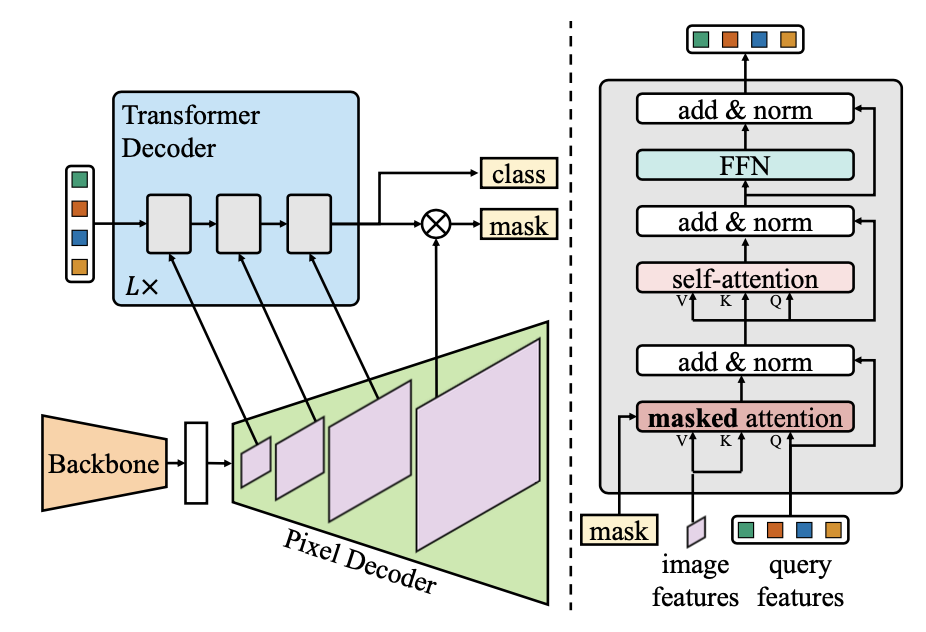
\includegraphics[width=\linewidth]{15.png}
	\caption{Mask2Former 网络结构图}
	\label{fig:fig15}
\end{figure}

为了解决这种分割问题,最近的工作试图设计通用架构,能够用相同的架构处理所有分割任务(即通用图像分割)。这些结构通常基于端到端集预测目标(例如,DETR),并在不修改结构、损失或训练过程的情况下成功地处理多个任务。尽管具有相同的体系结构,但通用结构仍然针对不同的任务和数据集分别进行训练。尽管现有的通用结构足够灵活,可以处理任何细分任务,但在实践中,它们的性能落后于最好的专用结构。除了性能较差之外,通用结构也更难训练。他们通常需要更先进的硬件和更长的训练时间。性能和训练效率问题都阻碍了通用结构的部署。

Masked attention Mask Transformer(Mask2Former) \cite{DBLP:conf/cvpr/ChengMSKG22}作为通用的图像分割体系结构可以在不同的分割任务中都优于专用的结构,同时在每个任务上都很容易训练。如 \textbf{图 \ref{fig:fig15}} 所示,模型由从图像中提取低分辨率特征的主干网络;从主干输出中逐渐向上采样低分辨率特征,以生成高分辨率的每像素嵌入的像素解码器;对图像特征进行操作以处理对象查询的Transformer解码器三部分组成。

 K-Net \cite{zhang2021k}是一种通过一组可学习的核来统一图像分割(语义分割、实例分割)的方法。这些来自 K-Net 的可学习的核可以在视频帧中自然地关联相同的实例。基于 K-Net,Video K-Net \cite{li2022video}通过简单的基于核的外观建模和跨时间内核交互,学会了同时分割和跟踪视频中的``things''和``stuff''(语义分割和实例分割),实现了简单、强大、统一的端到端视频全景分割框架。在Citscapes VPS 和 KITTI-STEP 上实现了最先进的视频全景分割结果。可以看到,无论是在图像分割还是在视频分割领域,通用的分割框架是当下的一个研究热点。
\section{总结}
\label{sec:conclusion}

传统数字图像处理方法使用成熟的技术处理问题,如特征描述子(SIFT、SUR、BRIEF 等)。在深度学习兴起前,图像分类等任务需要用到特征提取步骤,特征即图像中``有趣''、描述性或信息性的小图像块。这一步可能涉及多种数字图像处理算法,如边缘检测、角点检测或阈值分割算法。从图像中提取出足够多的特征后,这些特征可形成每个目标类别的定义(即``词袋'')。部署阶段中,在其他图像中搜索这些定义。如果在一张图像中找到了另一张图像词袋中的绝大多数特征,则该图像也包含同样的目标(如椅子、马等)。传统方法的缺陷是从每张图像中选择重要特征是必要步骤。而随着类别数量的增加,特征提取变得越来越麻烦。要确定哪些特征最能描述不同的目标类别,取决于研究人员的判断和长期试错。此外,每个特征定义还需要处理大量参数,所有参数必须由人来进行调整。

而深度学习的快速发展和设备能力的改善(如算力、内存容量、能耗、图像传感器分辨率和光学器件)提升了视觉应用的性能和成本效益,并进一步加快了此类应用的扩展。与传统方法相比,深度学习可以帮助 研究人员在图像分类、语义分割和目标检测等任务上获得更高的准确率。由于深度学习所用的神经网络是训练得到而非编程得到,因此使用该方法的应用所需的专家分析和微调较少,且能够处理目前系统中的海量可用视频数据。深度学习引入了端到端学习的概念,即向计算机提供的图像数据集中的每张图像均已标注目标类别。因而深度学习模型基于给定数据``训练''得到,其中神经网络发现图像类别中的底层模式,并自动提取出对于目标类别最具描述性和最显著的特征。

但这并不意味着传统方法的没落,在本文的调研和分析中,可以看到即使在深度学习大放异彩的时代,仍在一定程度上依赖于传统方法的使用,甚至从中获得理论指导或思路启迪,如正交变换、高斯滤波等。传统数字图像处理方法和深度学习方法之间存在一定的权衡。传统方法成熟、透明,且为性能和能效进行过优化;深度学习提供更好的准确率和通用性,但消耗的计算资源也更大。混合方法结合传统方法和深度学习,兼具这两种方法的优点,更加适用于需要快速实现的高性能系统。



% Can use something like this to put references on a page
% by themselves when using endfloat and the captionsoff option.
\ifCLASSOPTIONcaptionsoff
  \newpage
\fi



{\small
\bibliographystyle{IEEEtran}
\bibliography{reference/egbib}
}

% that's all folks
\end{sloppypar}
\end{document}


